\documentclass[article,a4paper,twoside]{memoir}
\usepackage{graphicx,textcomp,authblk,wallpaper,xcolor}
\usepackage{amsmath,amssymb,amsfonts,hyperref,tikz}
\usepackage[T1]{fontenc}

% JA: Is this used?
%\usepackage{mathrsfs}`
\usepackage{relsize}
\let\acr=\textsmaller

\newcommand{\C}[1]{\ensuremath{\mathrm{C}_{#1}}}

\counterwithout{section}{chapter}
\setsecnumdepth{subsubsection}

\setlength{\parindent}{0em}
\setlength{\parskip}{0.7em}
\setlrmarginsandblock{2.4cm}{2.4cm}{*} 
\setulmarginsandblock{2.4cm}{2.7cm}{*}
\checkandfixthelayout

\definecolor{green}{rgb}{.2,.35,.1}
\definecolor{blue}{rgb}{.1,.2,.4}
\newcommand{\program}[1]{\textit{#1}}
\newcommand{\filename}[1]{\texttt{#1}}
\newcommand{\funname}[1]{{\color{blue}\textbf{#1}}}
\newcommand{\paramname}[1]{{\color{green}\textbf{#1}}}

\aliaspagestyle{title}{empty}

\title{\program{Fullerene} (Version 4.5) \\A Program for the Topological Analysis of Fullerenes \\ User's Manual}

\author{Peter Schwerdtfeger%
  \thanks{Email: \texttt{p.a.schwerdtfeger@massey.ac.nz}}
}
\author{Lukas Wirz%
  \thanks{Email: \texttt{l.wirz@massey.ac.nz}}
}
\affil{Centre of Theoretical Chemistry and Physics, The New Zealand Institute
 for Advanced Study, Massey University Auckland, Private Bag 102904,
 North Shore City, \\
 0745 Auckland, New Zealand.}

\author{James Avery%
  \thanks{Email: \texttt{avery@nbi.ku.dk}}
}
\affil{Niels Bohr Institute, University of Copenhagen, 2100 Copenhagen, Denmark.}

\preauthor{
  \begin{center}
    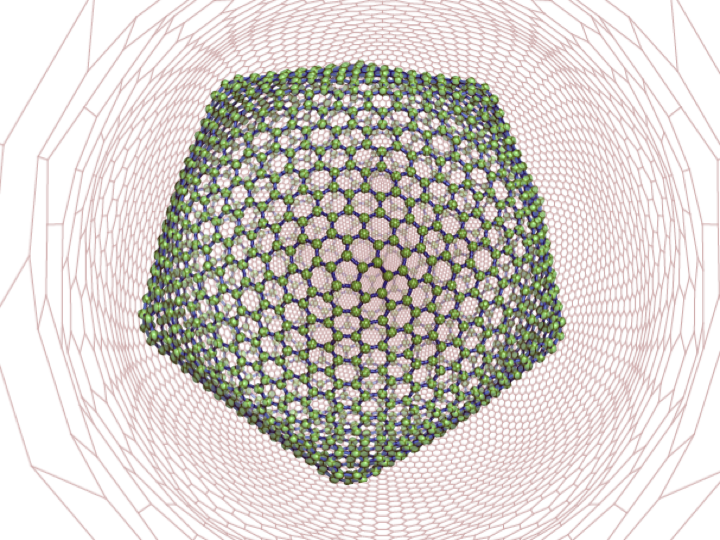
\includegraphics[width=0.9\textwidth]{Toc.png}
    \large \lineskip 0.5em%
    \begin{tabular}[t]{c}
}

\begin{document}

\maketitle

\cleardoublepage

\section*{Important Copyright Message:}
\textit{This is an \textbf{open-source code} and you may use and modify the program at your own will.
If you like to know why, read the article by \textrm{Darrel C. Ince, Leslie Hatton, 
John Graham-Cumming, Nature \textbf{482}, p.485 (2012)}. However, we kindly ask that if 
our program is used, and data are subsequently published, to cite the references given below.
Before you distribute the program to other agencies or users outside your
group/department please make them aware that their name should be
added into our user's database. For more details go to our website at Massey University:}
{

 \centering
  \url{http://ctcp.massey.ac.nz/index.php?group=&page=fullerenes&menu=fullerenes}

}
For any questions concerning this program please feel free to contact us.
We are always open to improvements and suggestions.

\subsubsection*{Please cite the following paper if you use this program for publishing data:}
\begin{enumerate}
	\tightlist
	\item P. Schwerdtfeger, L. Wirz, J. Avery, \textit{\program{Fullerene} -- A Software
	 Package for Constructing and Analyzing Structures of Regular Fullerenes}, J. Comput. Chem. \textbf{34}, 1508--1526 (2013).
\end{enumerate}
\subsubsection*{We also recommend to cite the following book (many of the concepts used can be found here):}
\begin{enumerate}
	\setcounter{enumi}{1}
	\tightlist
	\item P. W. Fowler and D. E. Manolopoulos, \textit{An Atlas of Fullerenes}
	(Dover Publ., New York, 2006). This book is highly recommended. It helps understanding how this program functions.
\end{enumerate}
\subsubsection*{Further suggested reading:}
\begin{enumerate}
	\setcounter{enumi}{2}
	\tightlist
	\item P. Schwerdtfeger, L. Wirz, J. Avery, \textit{The Topology of Fullerenes}, WIRE Comput. Mol. Sci. \textbf{5}, 96--145 (2015).
	 \item L. N. Wirz, R. Sure, R. Tonner, A. Hermann, P. Schwerdtfeger, \textit{A Harmonic Force-Field Method for Fullerenes and a Comparison to Density Functional Calculations for Goldberg-Coxeter Fullerenes up to C$_{980}$}, J. Comput. Chem., in press.
	\item D. Babi\'c, \textit{Nomenclature and Coding of Fullerenes}, J. Chem. Inf. Comput. Sci. \textbf{35}, 515--526 (1995).
	\item D. E. Manolopoulos and P. W. Fowler, \textit{Molecular graphs, point groups, and fullerenes}, J. Chem. Phys. \textbf{96}, 7603--7614 (1992).
	\item Z. C. Wu, D. A. Jelski, and T. F. George, \textit{Vibrational Motions of Buckminsterfullerene}, Chem. Phys. Lett. \textbf{137}, 291--295 (1987).
	\item G. B. Adams, M. O'Keefe, and R. S. Ruoff, \textit{Van der Waals Surface Areas and Volumes of Fullerenes}, J. Phys. Chem. \textbf{98}, 9465--9469 (1994).
	\item G. Brinkmann, P. W. Fowler, \textit{A Catalogue of Growth Transformations of Fullerene Polyhedra}, J. Chem. Inf. Comput. Sci. \textbf{43}, 1837--1843 (2003).
	\item D. Babi\'c, D. J. Klein and C. H. Sah, \textit{Symmetry of fullerenes}, Chem. Phys. Lett. \textbf{211}, 235--241 (1993).
	\item T. Pisanski, B. Plestenjak, and A. Graovac, \textit{NiceGraph Program and its applications in chemistry}, Croatica Chemica Acta \textbf{68}, 283--292 (1995).
	\item B. Plestenjak, \textit{An algorithm for drawing Schlegel diagrams}, \url{http://www-lp.fmf.uni-lj.si/plestenjak/Papers/NICEGR.pdf}.
	\item J. Bondy and U. Murty, \textit{Graph Theory} (Springer, Berlin, 2008).
	\item A. J. M. Wilson, \textit{Graphs and Applications. An Introductory Approach} (Springer, Berlin, 2000).
	\item J. Cioslowski, N. Rao, and D. Moncrieff, \textit{Standard Enthalpies of Formation of Fullerenes and Their Dependence on Structural Motifs}, J. Am. Chem. Soc. \textbf{122}, 8265--8270 (2000).
	\item M. Alcam\'i, G. Sanchez, S. Diaz-Tendero, Y. Wang, F. Martin, \textit{Structural Patterns in Fullerenes Showing Adjacent Pentagons: \C{20} to \C{72}}, J. Nanosci. Nanotech. \textbf{7}, 1329--1338 (2007).
	\item F. Cataldo, A. Graovac, O. Ori \textit{The Mathematics and Topology of Fullerenes} (Springer, Berlin, 2011).
\end{enumerate}

\clearpage

\tableofcontents
\begin{center}
\line(1,0){350}
\end{center}

\vspace{1cm}
%Figure 6
 \begin{figure}[htbp]
	\centering
  		 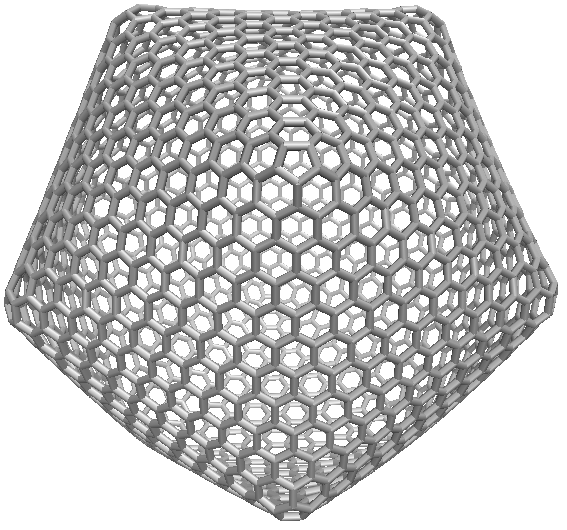
\includegraphics[width=0.6\textwidth]{C2160.png}
     \caption{Force-field optimized structure of $I_h$-\C{2160} viewed with VMD \cite{vmd}.}
     \label{pic:Finalgraph}
 \end{figure}

\vspace{2cm}
\textbf{Acknowledgement:} \textit{PS is indebted to the Alexander von Humboldt Foundation (Bonn) for financial support 
in terms of a Humboldt Research Award, and to both Prof. Gernot Frenking and 
Dr. Ralf Tonner (Marburg) for support during his extended stay in Marburg where 
writing of this program began. We acknowledge the help of Darko Babi\'c, Patrick 
W. Fowler (Sheffield) and David E. Manolopoulos (Oxford) for permission to freely distribute 
their Fortran subroutines which we modified and implemented in this program package.
We also thank Prof. Ottorino Ori (Zagreb) and Jan Goedgebeur (Gent) for fruitful discussions.}

\clearpage

%Introduction
\section{Introduction}
\textit{Fullerene} is a general purpose computer program that creates the adjacency matrix
for any fullerene isomer, performs a topological/graph theoretical analysis, and
creates a reasonably accurate 3D structure (cartesian or internal coordinates) through
various different methods and algorithms. The results can be used for plotting 2D
fullerene graphs (e.g., Schlegel diagrams) and 3D structures, and serves as a good
starting point for further quantum theoretical treatment.  The program is written
in standard Fortran and C++ and is easily implemented within a Linux/\acr{UNIX}
environment.  Although there are several other computer programs already available
to deal with fullerene graphs like \program{CaGe}(\program{plantri},\cite{Brinkmann05}
\program{fullgen},\cite{Brinkmann} \program{Buckygen}\cite{Goedgebeur,Goedgebeur1}),\cite{Brinkmanx}
\program{Vega},\cite{Pisanski}, \program{FuiGui},\cite{FuiGui} or the routines introduced
in the book by Fowler and Manolopoulos,\cite{Atlas} we felt that there is a need
to write a general purpose program which does what other programs do and (of course)
a lot more.  The first version (1.0) was written in Fortran for calculating the
surface area and volume of a fullerene and corresponding changes due to endohedral
incorporation of rare gas atoms \cite{Tonner}.  A much improved version 2.0 allowed
for the creation of fullerene structures using the ring-spiral algorithm introduced
in the book by Fowler and Manolopoulos \cite{Atlas}, and version 3.0 was already
dealing with topological and graph theoretical properties.  It became soon clear
that many open problems remain in fullerene structure generations which needed to
be addressed,\cite{WIRE2015} and it was therefore decided to extend version 3 to a general purpose
program package and make it available to the scientific community.\cite{Schwerdtfeger2013}

In the current version only regular fullerenes are considered (i.e. of genus~0 consisting
of pentagons and hexagons only) fulfilling Euler's theorem, $n_v - n_e + n_f = 2$,
where $n_v$ is the number of vertices (atoms), $n_e$ the number of edges (bonds),
and $n_f$ the number of faces (5- or 6-rings). The program constructs an accurate
3D structure (in cartesian coordinates) of any fullerene isomer from the canonical
ring spiral pentagon indices (RSPI) (or its generalized version) through either a 3D Tutte embedding (3D-TE) \cite{Tutte}
or the adjacency matrix eigenvector (AME) method \cite{Atlas}. One can also construct
the $n$-th leapfrog $GC_{1,1}^n[C_{n_v}]$ fullerene, the halma fullerene $GC_{k,0}[C_{n_v}]$
or the more general Goldberg-Coxeter transformation of a fullerene $GC_{k,l}$
with $k \geq l$, which is implemented not only for \C{20}, i.e. $GC_{k,l}[C_{20}]$, as in a
previous version (4.4) of the program, but also for any fullerene using an algorithm developed
by Avery.\cite{Avery2015}
Starting from a given fullerene structure one can perform vertex insertions (such
as Endo-Kroto \cite{Endo92}, Yoshida-Fowler \cite{Yoshida97a} or Brinkmann-Fowler \cite{BrinkmannFowler03})
or Stone-Wales transformations \cite{Stone86}.  Vertex insertions allow for the
construction of non-spiral fullerenes such as \C{380} or \C{384}.  Geometry optimization
using a Fletcher-Reeves-Polak-Ribiere minimization \cite{NumRec} with analytical
gradients for the harmonic oscillator force field \cite{Wu87,Wirz2015} is implemented in the
current version, providing a good initial guess for 3D cartesian coordinates.  2D~fullerene
graphs (e.g. Schlegel diagrams) can be produced using a variety of different algorithms \cite{Plestenjak}.
The program determines the volume and surface area of a fullerene (irregular or
not) through tesselation in trigonal pyramids or from its convex hull, and gives
measures for spherical distortion and convexity.  It determines the minimum covering
sphere, the minimum distance sphere and the maximum inner sphere.  The program further
calculates the number of Hamiltonian cycles and produces ring spiral indices.  Cioslowski's
scheme for the calculation of the heat of formation for IPR (isolated pentagon rule)
fullerenes is implemented \cite{Cioslowski2000}, as well as Babi{\'c}'s scheme for
calculating the total resonance energy of a general fullerene \cite{Babic1995,Babic1997},
and Martin's scheme for the heat of formation \cite{Alcami}.  A variety of topological
indicators, such as the Wiener index, Szeged index and Balaban index are calculated.\cite{Wiener1947,Balaban}

This program works for any (distorted or not) regular fullerene. The spiral algorithm of Fowler and Manolopoulos used here \cite{Atlas}
is not restricted to a pentagon start or to canonical indices. For a general list of fullerenes see ``The House of Graphs'' \cite{HouseofGraphs}. 
The program produces an external file with default name \filename{Fullerene-3D.xyz} or \filename{Fullerene-3D.cc1}
to be used for standard molecular plotting programs
like CYLview \cite{CYLview}, Avogadro \cite{Avogadro}, Jmol \cite{JMol}, Pymol \cite{Pymol} or VMD \cite{vmd}.  For using these programs 
it is important that the fullerene has a reasonable 3D structure, obtained for example by a force field 
optimization, otherwise bonds cannot be correctly identified from the .xyz file only. It may therefore not
be advisable to use structures that come out directly from
the AME or 3D-TE algorithm, or the .cc1 file could be used containing information on vertex adjacencies. 
We recommend VMD \cite{vmd}, it is more robust and works even for the largest fullerenes beyond 1000 atoms. The program produces fullerene 2D graphs 
in latex format, but can be used by any other program which is capable of producing 2D graphs, for example QMGA \cite{Gabriel2008}. 
For this an external file is written out called \filename{Fullerene-2D.dat} containing all the information required for plotting a 2D graph.

From version 4.0 onwards (released July 2012) C++ routines embedded into the original Fortran program incorporate
much improved algorithms compared to the older versions. The reason for using two different program languages is
that PS is good in old-fashioned Fortran, JA is good in C++ (and LW is doing both).  Furthermore, some of the original routines used were available 
in Fortran only. Some standard routines from Mathematical Recipes were modified for the purpose of matrix diagonalization 
and geometry optimization. Version 4.3 included the Hessian of the force field, and in this version (4.5) 
force constants are used which match experimental or calculated vibrational frequencies.
Version 4.4 introduced a search algorithm for neighbourhood RSPIs, the Szeged index, pentagon arm indices as further topological descriptors,
and new (conjectured) upper and lower bound for Hamiltonian cycles in fullerenes.
Version 4.5 has a new algorithm for general Goldberg-Coxeter transforms \cite{Avery2015}.
The Tutte embedding algorithm has also been optimized to perform much faster, and the fullerene database has been transformed into a more compact and efficient version.
Version 5 to be released late 2016 will separate the topological from the cartesian input part and uses sparse matrix handling for the
largest fullerenes. This program is under permanent construction and has been tested extensively for bugs.
Nevertheless, if you have any problem or find any bugs please report to one of us.

There are many things on our to-do list. We try hard to release more functionality to this program in due time.
Not implemented yet is: 

\begin{itemize}
\tightlist
\item The minimum covering ellipsoid useful for rugby-ball shaped fullerenes, and
close packing of ellipsoids;
\item Symmetrization of optimized coordinates to point group symmetry (or a chosen
lower symmetry) and symmetry labels for H\"uckel orbital energies and vibrational frequencies;
\item Extension to general cubic polyhedra of genus~0 (heptagons and squares); 
\item Extension to non-regular fullerenes of higher genus;
\item A restart option for subroutine Hamilton as it is an $\#P$-hard problem and
we like to test the limitations of the back-track algorithm used in program;  
\item Kekul\'e structures (perfect matchings, so far only the counting is implemented) and Clar sextets;
\item General plotting program (other than latex) for producing Schlegel diagrams
and corresponding duals with a good graphical interface similar to the \program{CaGe} program;\cite{Brinkmanx}
\item Further extension of the fullerene database.
\item Implementation of the Brinkmann-Goedgebeur fast-generation algorithm for fullerenes,
which is more efficient than the original ring-spiral code of Fowler and Manolopoulos.
\end{itemize}

We are also open to any other suggestions and welcome additions to this program suite.
In this case please feel free to contact us per email.

 \begin{figure}[htbp]
   	\centering
  	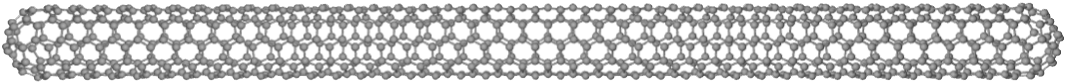
\includegraphics[width=\textwidth]{C840.png}
%    \label{pic:toc}
 \end{figure} 
 
\clearpage
%Installation and running the program
\section{Installation and running the program}
All fortran source files are located in the directory ``source'' and all C++ files are in ``libgraph''.

The program is Linux/\acr{UNIX} based and is tested to compile with the gnu compiler collection (more specifically gfortran and g++).
You need to use the \filename{Makefile} included in the \filename{fullerene.zip} file provided and type\\\\
\verb|make|

In the Makefile several compile flags are set.  Per default, the machine dependent flag \verb|-m64| is set (if you are
using a 32-bit environment you will need to change this to \verb|-m32|).  The optimization level is set to \verb|-O3|.  
If you require an atom count above 5000 (the upper limit can be set in \filename{source/config.f}, see entry \paramname{Nmax=5000})
there will be arrays which are larger than 2\,GB.  Per default most compilers don't support this. 
If your machine has enough memory, your gfortran is sufficiently new
(4.4.3 to 4.4.7  and 4.6 on 64-bit Linux work) you can set \verb|-mcmodel| to \verb|medium| to switch to the medium code model in
which objects are permitted to be larger than 2\,GB (on Macs this may not always work).  All binary objects must be compiled with the same options; delete all
binaries before you recompile using a different code model. 

The executable ``fullerene'' can be executed on a Linux/\acr{UNIX} as\\\\
\verb|./fullerene < filename.inp > filename.out|

A number of test input files can be found in the directory ``input''. If you type\\\\
\verb|make tests|

it will run all the input jobs and stores them into the output directory as *.out. If you type\\\\
\verb|make clean|

all the object files are deleted. Additionally, the linked binaries are deleted if you type\\\\
\verb|make distclean|

All input and output files provided have been checked for correctness. The test files will run a couple of minutes
on a fast intel processor.

If you use our fullerene database (which is recommended for time savings), the directory \filename{database} needs 
to be created (if not already there) and moved into the main directory where the \filename{source} and \filename{libgraph} 
directories are located. Please download our databases and move it into this folder. \filename{database} should contain
the folders \filename{ALL} with our database for general fullerenes, \filename{IPR} with our database 
for IPR fullerenes, \filename{Yoshida} with Yoshida's database of selected fullerenes (directories containing .cc1 files),
and \filename{HOG} with (if downloaded from http://hog.grinvin.org/Fullerenes ) the House of Graph data files. Important: 
Please make all filenames in the database read-only.

To use the latex program for the 2D fullerene graphs you need to use the files \filename{standalone.cfg} and \filename{standalone.cls}.

\clearpage
%Program Structure
\section{Program Structure}
The main program (\filename{main.f}) calls a number of subroutines for certain tasks and in a certain sequence (see Figure \ref{pic:flow_long}).
Subroutine \funname{DataIn} manages all the input and determines these main tasks to be carried out.
The input is in \textit{Namelist format} if not otherwise stated. 
Important steps in the program are given in Figure \ref{pic:flow_long} and are
explained in some detail in this section. Figure \ref{pic:flow_short} visualizes the workflow in a more abstract way.
More information can be obtained in our review article \cite{WIRE2015}.

%Figure 1
\begin{figure}[htbp]
   	\centering
	\includegraphics[]{tree.pdf} 
    \caption{Flow diagram for main program tasks.}
    \label{pic:flow_long}
\end{figure}

%Figure 2
\begin{figure}[htbp]
   	\centering
	\includegraphics[]{workflow.pdf} 
    \caption{Simplified diagram of the workflow.}
    \label{pic:flow_short}
\end{figure}

The most time-consuming steps in the program are the diagonalization of the adjacency matrix 
of the fullerene graph $F$, $A(F)$  
(needed for the AME algorithm and the H\"uckel analysis ($\mathcal{O}(n^3)$)), the force-field optimization for
very large fullerenes ($>$ 2000 atoms)  and the diagonalization of
the force-field Hessian, the determination of the number of Hamiltonian cycles
($>$ 80 atoms) (this is a $\#P$-hard problem), the creation of a list of ring-spiral pentagon
indices for all possible isomers with a given vertex count $n_v$ ($>$ 80 atoms), 
and the Tutte embedding algorithm ($>$ 2000 atoms). We try to improve the performance of these algorithms
in our next major version to be released. For version 4.1 the fullerene database was increased and a link to
the House of Graphs was introduced. Version 4.2 saw the introduction of dihedral angles into the force field,
and Version 4.3 was extended to calculate frequencies from the force-field Hessian, and Version 4.4 saw
the implementation of the Goldberg-Coxeter transformation $GC_{k,l}$ of \C{20} for all possible combinations of $k \geq l$,
new topological descriptors and a more compact version of the database. Version 4.5 removed some of the bugs and includes
a general Goldberg-Coxeter transformation $GC_{k,l}[C_n] ~(k\ge l, l\ge 0)$ of any fullerene. Version 4.5 also has optimized 
force constants for a frequency analysis.

%there should a subsection "creation of the fullerene graph" in this place
%\subsection{Create a 3D structure for a specific fullerene}

%Create a 3D structure for a specific fullerene
\subsection{Create a 3D structure for a specific fullerene}

The easiest way to create a 3D structure for \program{Fullerene} is of course to read-in cartesian coordinates for a specific
fullerene (see input files \filename{CCc20.inp} to \filename{CCc540.inp}), or to construct them internally for the high
symmetry $I_h-$\C{20} or $I_h-$\C{60} isomers (Subroutine \funname{CoordC20C60}, see input files \filename{GEOMc60.inp},
\filename{GEOMc60exp.inp}, \filename{GEOMc60ideal.inp}), or to construct the cartesian coordinates from a generalized ring-spiral
pentagon-indices RSPI (plus jumps if necessary) by using either the Fowler-Manolopoulos AME algorithm \cite{Atlas},
or the more reliable 3D-TE algorithm (Subroutine \funname{CoordBuild}, see input files \filename{RSPIc20.inp} or \filename{RSPIc840.inp}),
or from a Goldberg-Coxeter 2-index transformation of \C{20}, i.e. $GC_{k,l}(20)$ with $k \geq l$ and $k > 0$
(triangulation algorithm described below, see input files \filename{GEOMc20Halma.inp}, \filename{GEOMc500Halma.inp}) or \filename{GGCK6L2.inp}). 
The 12 pentagon indices can also be obtained from the \textit{fullerene database} using 
the canonical fullerene number as defined in the book ``Atlas of Fullerenes'' by Fowler and Manolopoulos \cite{Atlas,cvetkovic2002} 
(e.g. input file \filename{DBc66.inp}). Information of vertex connections (edges) can also be used as input 
(input files \filename{EDGEc20.inp} and \filename{EDGEc60.inp}).
The program prints internal coordinates in form of a $Z$-Matrix (distances, angles and dihedrals).
For this the atoms are rearranged (permuted) such that the distances are smallest. Note that this works well for optimized
coordinates, e.g. cartesian coordinates obtained from a force-field optimization.

In addition to the original ring spiral algorithm by Fowler and Manolopoulos we
have implemented a general ring spiral algorithm for cubic graphs.  It
differs from the classical ring spiral algorithm in that it can insert
jumps between the addition of two vertices to the spiral in order to
prevent walking into a cul-de-sac at a later stage.  It is therefore
capable of describing all fullerene graphs (and any other cubic graph).
The criterion for jumping (while deriving the spiral from a graph) is,
that the subgraph that hasn't been added to the spiral yet, must never
be disconnected.  For deriving the graph from the spiral it is necessary
to explicitly give the jump positions and distances. 

We recommend reading Fowler and Manolopoulos' book \cite{Atlas,cvetkovic2002} for
the use of RSPIs and H\"uckel (adjacency matrix) $P$-type eigenvectors to construct
3D fullerene graphs.  For the Goldberg-Coxeter transformation of \C{20} we obtain
the RSPI from the scheme introduced by Fowler and Rogers.\cite{Rogers}  For the AME
algorithm it is critical to get the right H\"uckel eigenvectors for the construction
of cartesian coordinates,\cite{Atlas} which worked well for the icosahedral fullerenes,
but less well for fullerene nanotubes.  The position of the three~$P$-type eigenvectors
can be specified (see file \filename{RSPIc60NT.inp} for such an example).  If the
AME algorithm fails or you cannot find the required $P$-type eigenvectors, you should
use our Tutte embedding algorithm, which (to our opinion) is less troublesome and
may be used as the standard method to construct 3D structures.  The disadvantage
of this algorithm is, however, that the structure could be far off from a force-field
optimized global minimum for a fullerene, and the force-field optimization might
end up in a heavily distorted unreasonable 3D local minimum (for strategies to avoid
this see the input section).

It is important that the end-product is viewed by a molecular
visualization program.  We recommend CYLview by Claude Legault
\cite{CYLview}, Avogadro \cite{Avogadro}, JMol \cite{JMol}, Pymol
\cite{Pymol} or VMD \cite{vmd}.  Most of these programs are freely
available.  For this purpose a file is written to Fullerene-3D.xyz or
Fullerene-3D.cc1 to be used as an input file for the various molecular
visualization programs available.

The program sets the barycenter of the fullerene 
to the origin. Using the obtained cartesian coordinates the program calculates the smallest and largest cage diameters and the
moment of inertia, which already gives a measure for distortion from spherical symmetry (Subroutine \funname{Diameter}). 
It produces the distance matrix~ $d_{ij}$ if the print level is set to high (Subroutine \funname{DistMatrix}), and once the 
molecular point group is obtained, the program determines if the fullerene is chiral or not (Subroutine \funname{Chiral}).
Once the cartesian coordinates $(X_i, Y_i, Z_i)$ for each vertex $i=1,\dots, n_v$ is known, all edges are determined by 
analyzing connectivities between the vertices from either given cartesian coordinates or directly from the adjacency matrix 
if a ring spiral input was chosen (Subroutine \funname{Connect}). In any case, one has the adjacency matrix $A_{ij}$ for all vertices at this stage:
\begin{equation}
  \label{eq:adjacencymatrix}
  A_{ij} =
  \begin{cases}
    1 & \text{if vertices $i$ and $j$ are adjacent}\\
    0 & \text{otherwise}
  \end{cases}
\end{equation}

%List of Isomers
\subsection{List of Isomers}
The program can print all general and IPR isomers for a specific fullerene and perform an analysis as introduced 
in the book by Fowler and Manolopoulos \cite{Atlas}, e.g. pentagon indices and 
pentagon number, hexagon indices and strain parameter, NMR information and number of distinct Hamiltonian cycles if 
required. The number of isomers scales polynomially as $n_v^9$, thus it becomes computationally
very demanding to produce a full isomer list for fullerenes larger than \C{120}. Moreover, the database provided, can be used to print all isomers up to 
\C{140}, and up to \C{184} for all IPR isomers. Fowler and Manolopoulos use a numbering scheme ($N_\mathrm{isomers}= 1,\dots, n_\mathrm{max}$) 
obtained from the natural sequence of canonical RSPIs to distinguish between the different isomers \cite{Atlas}. From their book \cite{Atlas} the
general isomer number can be taken and the RSPIs for a specific isomer up to \C{150} can be read-in from the database provided. 
The numbering scheme for IPR isomers only ($N_\mathrm{isomers}^\mathrm{IPR}= 1,\dots, n_\mathrm{max}$) can also be used up to \C{200}, 
see for example the input file \filename{DBc158.inp}.

%H\"uckel analysis and topological indicators
\subsection{H\"uckel analysis and topological indicators}
From the adjacency matrix $A_{ij}$ of eq.(\ref{eq:adjacencymatrix}), a H\"uckel analysis
is performed (Subroutine \funname{Hueckel}).  This gives you a good hint if the fullerene
is of open or of closed shell \cite{Atlas}.  For smaller fullerenes or non-IPR fullerenes,
the H\"uckel analysis may not be very reliable as hybridization with the C(2s) orbitals
occurs due to non-planarity.  Hence the $\sigma-\pi$ separation breaks down.  The
orbital energies are defined as
\begin{equation}
  \label{Hueckel}
  \epsilon_i=\alpha+x_i\beta
\end{equation}
and we adopt $\alpha = -0.21$ au  and  $\beta = -0.111$ au obtained from the experimental
ionization potential (7.58 eV) and excitation energy (3.02\,eV) of \C{60} (NB: the
electron goes into the second LUMO of $t_{1g}$ symmetry).  This gives also orbital
energies for \C{60} in reasonable agreement with DFT Kohn-Sham orbital energies.
The fullerene structure might also undergo a Jahn-Teller distortion adopting a singlet 
ground state instead of one of a higher multiplicity, as this is the case for \C{20}.
Such electronic effects are not captured in this program, and one needs to perform
a proper quantum-theoretical calculation. The program gives information on the HOMO-LUMO
gap and calculates the topological resonance energy from Babi\'c's matching polynomial
calculations \cite{Babic1995,Babic1997}.

A topological index is a structurally invariant natural or real number related to
a molecular graph, which does not depend on the labelling or the 2D representation
of a graph $G$.  There are several other topological indicators \cite{Cataldo,Caporossi}
of which the Estrada index, the Wiener index, the hyper-Wiener index, the Balaban
index, the Szeged index, the topological radius, diameter and and mean distance are
printed.

The Estrada $E(G)$ and bipartivity $\beta(G)$ indices are obtained from
the eigenvalues of the adjacency matrix $A(G)$, $\{ x_i, i=1,\ldots,n_v \} \in [-3,3]$,
of a graph $G$ (in our case a regular fullerene graph $G=F$) \cite{Estrada,Doslic2005},
\begin{equation}
  \label{Estrada}
  E(G)=\sum_{i=1}^{n_v}e^{x_i} \quad \text{ and } \quad \beta(G)=\sum_{i=1}^{n_v}\cosh(x_i)/E(G)
\end{equation}
The Estrada index for $I_h$-\C{60} is $E$= 197.450228 and the corresponding bipartite index $\beta$= 0.992966.

The Wiener $W(G)$ and hyper-Wiener $WW(G)$ indices are defined as \cite{Wiener1947},
\begin{equation}
  \label{Wiener}
  W(G)=\frac{1}{2} \sum_{\{ i,j \} \subseteq V(G)} D_{ij} \quad \text{ and } \quad WW(G)=\frac{1}{2} \sum_{\{ i,j \} \subseteq V(G)} \left( D_{ij} + D_{ij}^2 \right)
\end{equation}
Here, $V(G)$ is the vertex set and $D_{ij}$ is the topological (chemical) distance
matrix containing the topological distances between the two vertices $i$ and $j$,
i.e., the number of edges in the shortest path connecting them. 

For $I_h$-\C{60} we have $W(G)=8340$ and $WW(G)=27180$. If we define
\begin{equation}
  \label{TopDist}
  d_i^{\mathrm{max}} = \max\limits_{j} \{ D_{ij} \},
\end{equation}
we can define the topological diameters $D$ and radius $R$ as \cite{Caporossi}
\begin{equation}
  \label{TopDist}
  D = \max \{ d_i^\mathrm{max} \} \quad \text{ and } \quad  R = \min \{ d_i^\mathrm{max} \}.
\end{equation}
We can now define the reverse Winer index\cite{Balaban2000} as
\begin{equation}
  \label{RevWiener}
  W_\mathrm{rev} = n_v(n_v - 1)D/2 - W
\end{equation}
which for \C{60} is 7590.  The Balaban index is defined as \cite{Balaban},
\begin{equation}
  \label{Balaban}
  B(G)=\frac{n_e}{n_e-n_v+2} \sum_{i<j \in E(G)} \left( W(i)W(j) \right)^{-1/2}
\end{equation}
$n_e$ are the number of edges and $W(i)$ is the sum of topological distances between vertex $i$ and all other vertices in the graph,
\begin{equation}
  \label{sum}
  W_i=\sum_{j \in V(G)} D_{ij}
\end{equation}
For $I_h$-\C{60} we have $B(G)$= 0.910521583. The Schultz and Zagreb indices are also listed, although they are related to
the indices already defined here. The Szeged index is defined as\cite{Heydari}
\begin{equation}
  \label{Szeged}
  S_z(G)=\sum_{e \in E(G)} n_{i_j}(e)n_{j_i}(e)
\end{equation}
where $n_{i_j}(e) = |B_{i_j}(e)|$ is the number of vertices which are closer to vertex $i$ than vertex $j$ in an edge $e=(ij) \in E(G)$ (with
$E(G)$ being the edge set) and
\begin{equation}
  \label{Szeged1}
  B_{i_j}(e)= \{ k | k \in V(G), D_{ik} < D_{jk} \}
\end{equation}
Further listed are two topological efficiency parameters $\rho$ and $\rho_E$ defined by Vukicevic, Ori and co-workers \cite{Vukicevic,Ori},
\begin{equation}
  \label{rho}
  \rho=2\frac{W(G)}{n_v W_{\mathrm{min}}} \quad \text{ with } \quad W_{\mathrm{min}}= \min \{ W_i \}
\end{equation}
and
\begin{equation}
  \label{rhoE}
  \rho_E=\frac{W_{\mathrm{max}}}{W_{\mathrm{min}}} \quad \text{ with } \quad W_{\mathrm{max}}= \max \{ W_i \}
\end{equation}
For $I_h$-\C{60} both $\rho$ and $\rho_E$ are exactly 1.0. The spectral moments $\{ \mu_k, k=0,1,\dots \} $ are calculated from eigenvalues $x_i$ of the adjacency matrix,
\begin{equation}
  \label{specmom}
  \mu_k=\sum_{i=1}^{n_v} x_i^k
\end{equation}
and we have $\mu_0 = n_v$, $\mu_1 = 0$, $\mu_2 = 3n_v$, $\mu_3 = 0$, $\mu_4 = 15n_v$,
$\mu_5 = 120$, $\mu_4 = 93n_v - 120$, and $\mu_7 = 1680$.  The higher spectral moments
depend on the fullerene structure.\cite{Fowler93}

One of the first topological indicators introduced to discuss the stability of fullerenes
are the neighbour indices for pentagons and hexagons.  The program calculates the
pentagon neighbour indices,\cite{Atlas,Albertazzi} hexagon neighbour indices and
the pentagon arm indices.\cite{Reti}  Every fullerene isomer can be characterized
by a signature of the form $\{i_k | k=1, \dots, n\}$.  The pentagon indices $(p_i | i=0, \dots, 5)$
define the number of pentagons attached to another pentagon, i.e., for IPR fullerenes
$p_0 = 12$ and all other pentagon indices are zero.  Hexagon indices are similarly
defined, i.e., $(h_i | i=0, \dots, 5)$, where $h_k$ is the number of hexagons with
neighbour index $k$.  In an IPR fullerene every hexagon is adjacent to a minimum
of three others and we can restrict the list to $(h_3, h_4, h_5, h_6)$.  The pentagon
arm indices $(n_i | i=0, \dots, 5)$ counts the number of arms of the pentagons.  Here
an edge $E$ incident to a vertex of a pentagon not belonging to the pentagon is called
an arm if i) both end-vertices of edge $E$ are incident to pentagons, and ii) $E$ shares
two neighbour hexagons.\cite{Reti}  It is clear that this is nothing else than a
Stone-Wales pattern.

We can now define some useful topological invariants. The pentagon index $N_p$ is defined as
\begin{equation}
  \label{pentindex}
  N_p = \frac{1}{2}\sum_{k=1}^{5} kp_k \quad \text{ with } \quad  \sum_{k=0}^{5} p_k = 12
\end{equation}
For IPR fullerenes we have no pentagon attached to another and therefore $p_0 = 12$
and all other $p_i = 0$, and it follows that $N_p = 0$.  For IPR fullerenes a more
useful index is defined through the hexagon neighbour indices.  The standard deviation
$\sigma_h$ of the hexagon neighbour index distribution is defined as
\begin{equation}
  \label{standev}
  \sigma_h = \sqrt{\langle k^2 \rangle - \langle k \rangle^2}
\end{equation}
where
\begin{equation}
  \label{mean}
  \langle k^n \rangle = \frac{\sum_{k=1}^{6} k^n h_k}{\sum_{k=0}^{6} h_k}  \quad \text{ with } \quad  \sum_{k=0}^{6} h_k = \frac{n}{2} - 10
\end{equation}
R\'eti and L\'aszl\'o define the pentagon arm index $N_A$ in a similar way to the pentagon index,\cite{Reti}
\begin{equation}
  \label{arms}
  N_A = \frac{1}{2}\sum_{k=1}^{5} kn_k  \quad \text{ with } \quad  \sum_{k=0}^{5} n_k = 12
\end{equation}
The first and second moments $M_1$ and $M_2$ and the variance $\text{Var}$ are defined as (real numbers),
\begin{equation}
  \label{Moments}
  M_i = \frac{1}{12}\sum_{k=1}^{5} k^i n_k  \quad \text{ and } \quad  \text{Var}= M_2 - M_1^2
\end{equation}
We now define the R\'eti-L\'aszl\'o topological descriptor as $\Psi$,
\begin{equation}
  \label{Moments}
  \Psi = \frac{30+6M_1}{1+4.5N_p+C(M_1,M_2)} \quad \text{ with } \quad  C(M_1,M_2) = \frac{(120M_2)^{1/2}}{(1+7M_1)^{1/2}(1+0.9\text{Var}^{1.5})}
\end{equation}
If there exists a non-negative integer $q$ for which one of the arm indices $n_q = 12$,
the fullerene is called $q$-balanced.  In this case $\text{Var} = 0$.\cite{Reti}
If $N_p + N_A = 0$, the fullerene is called strongly isolated.  \C{60} contains Stone-Wales
patterns and is therefore not strongly isolated. The first leapfrog of \C{60}, \C{180},
and the ones to follow are strongly isolated.


%The Goldberg-Coxeter transformation
\subsection{The Goldberg-Coxeter transformation}

In a next step a Goldberg-Coxeter transformation $GC_{k,l}(n)$ for a fullerene \C{n} can be performed if required from the input
(Subroutine \funname{GoldbergCoxeter}). This leads to a fullerene C$_{k^2+kl+l^2}$. The current implementation allows only for
\textit{leapfrog transformations} ($k=l=1$) and for \textit{halma transformations} ($k \neq 0$ and $l=0$) for all fullerenes
(but all indices are allowed for $GC_{k,l}(20)$). A general $GC_{k,l}(n)$ for all values of $k$, $l$ and $n$ with $k \geq l$ 
is now implemented. 


%Figure 2
 \begin{figure}[htbp]
   	\centering
  	\includegraphics[]{gc}
    \caption{Goldberg-Coxeter construction: $GC_{1,1}$, leapfrog transformation; $GC_{3,0}$, halma transformation; $GC_{5,2}$, general.}
	\label{pic:GoldbergCoxeter}
 \end{figure}

The general Goldberg-Coxeter construction $GC_{k,l}[G_{0}]$ used here and shown in Figure \ref{pic:GoldbergCoxeter}
works in the following way: ($i$) Consider
a cubic planar graph $G_{0}$ and take its dual (faces become vertices and
vertices become faces), $D_{t}(G_{0})$. This transforms the graph $G_{0}$
with $n_v$ vertices into a triangulation, i.e. a geodesic sphere with $n_v$ triangles; (\textit{ii})
Each triangle $T_{k}$ ($k=1, \dots, n_{v}$) of the geodesic sphere is
tiled into another set of faces $t_i$ using the Coxeter indices ($k,l$).
If the obtained new smaller faces $t_i$ are not
triangles themselves within one $T_k$, when neighbouring $T_k$s are glued
together with other non-triangle faces, new triangles are formed and we end up with a new triangulation,
i.e. a larger geodesic sphere $GC_{k,l}D_{t}(G_{0})$;
(\textit{iii}) Finally we take the dual which yields a new fullerene,
\begin{equation}
 	G_1 = GC_{k,l}[G_0] = D_t[GC_{k,l} D_t(G_0)]
	\label{eq:GC}
\end{equation}

If the initial graph $G_0$ has $n_v$ vertices, the number of vertices of $GC_{k,l}[G_0]$ is
\begin{equation}
	n_v^{GC} = t(k,l)n_v = (k^2 + kl + l^2)n_v
	\label{eq:GCvertexcount} 
\end{equation}
$t(k,l)$ is called the {\em triangulation number}. We work with the dual triangulation instead of
a hexagonal mesh as it is easier to be implemented in a computer code.
This is shown in Figure \ref{pic:GoldbergCoxeter}. For icosahedral fullerenes ($I_h$ and $I$) with $l = k$ or $l = 0$, Fowler and Rogers 
showed how to construct the RSPIs,\cite{Rogers} which is implemented in this program as well for $GC_{k,l}(20)$. Figure \ref{pic:GK21C80} shows a $GC_{2,1}[\C{80}]$ transformation of a $D_{5d}$-\C{80} carbon nanotube transforming it into a chiral nanotube.

%Figure 2a
 \begin{figure}[htbp]
   	\centering
  	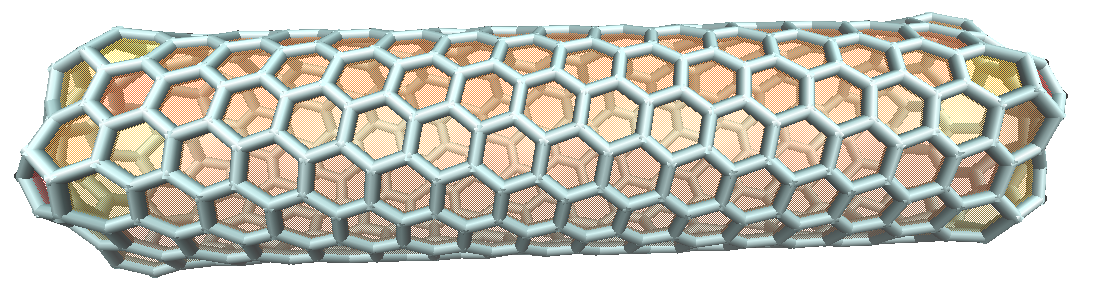
\includegraphics[width=0.6\textwidth]{GC(2,1)C80.png}
    \caption{Goldberg-Coxeter transformation $GC_{2,1}[\C{80}]$ transformation of a $D_{5d}$-\C{80} carbon nanotube into the chiral $D_{5}$-\C{560} nanotube.}
	\label{pic:GK21C80}
 \end{figure}
 
%Hamiltonian cycles
\subsection{Hamiltonian cycles}
Subroutine \funname{Hamilton} uses the back-track algorithm of Babi\'c \cite{Babic1995a} to obtain all 
Hamiltonian cycles and subsequently (if required) the IUPAC name of the fullerene. Hamiltonian cycles go through all vertices exactly once returning 
to the starting point. The number of distinct (non-isomorphic) Hamiltonian cycles has carefully been checked 
against a second algorithm developed by us for various fullerenes. Left-right cycles and cyclic vertex permutations count as the 
same cycle as they are isomorphic to each other. Although finding all Hamiltonian cycles is an NP-complete problem, the algorithm works fine up to about \C{100}. 
After that it becomes computationally very demanding as the algorithm scales like $O(2^{n_v})$. Therefore, for the larger fullerenes the program prints 
tight upper and lower limits for the number of Hamiltonian cycles instead. The existence of Hamiltonian cycles for fullerenes is only conjectured at this 
stage, and only for layered fullerenes (e.g. fullerene with onion-shaped 2D graphs such as nanotubes) existence has been proven. Our recent calculations verified that
Hamiltonian cycles exist for all fullerene isomers up to \C{120} and for all IPR isomers up to \C{122} \cite{PSAJDB}.

%Force-field optimization
\subsection{Force-field optimization}
The fullerene structure can be optimized by force fields using a Fletcher-Reeves-Polak-Ribiere geometry optimization \cite{NumRec}
with analytical gradients (Subroutine \funname{OptFF} \cite{NumericalRecipes}). In the current version the harmonic oscillator
force field (\acr{HOFF}) is implemented, which considers both bond lengths and angles only in an harmonic oscillator approximation \cite{Wu87}: 
\begin{multline}
  \label{eq:Ewu}
  E_{\mathrm{Wu}} = 
          \frac{k_p}{2} \sum_{i_p}^{\mathrm{p-edges}} \left(R_{i_p} - R_p\right)^2 
        + \frac{k_h}{2} \sum_{i_h}^{\mathrm{h-edges}} \left(R_{i_h} - R_h\right)^2 \\
        + \frac{f_p}{2} \sum_{j_p}^{60} \left(\theta_{j_p} - \theta_p\right)^2 
        + \frac{f_h}{2} \sum_{j_h}^{3\times n_v-60} \left(\theta_{j_h} - \theta_h\right)^2 
\end{multline}
Only bonded pairs of vertices are taken into account. $k_{p}$ and $k_{h}$ are
the force constants for the two different C--C bonds (set to $\approx 300 \text{\,kcal\,\AA}^{-2}$), $R_p$ and $R_h$ the corresponding pentagon and
hexagon bond distances ($\approx$ 1.4 \AA), and $\theta_p $ and $\theta_h$ are the corresponding bond angles (108$^\circ$ and 120$^\circ$
respectively). As the original Wu force field was developed for $I_h$-\C{60} only, adjacent pentagons are treated in the same way as a pentagon adjacent to a hexagon.

The \acr{HOFF} optimization is very fast even for fullerenes such as \C{840}. 
The \acr{HOFF} force-field optimization may lead to distortions of the fullerene to a structure of lower symmetry compared to the original point-group. 
Moreover, as no dihedral angles are fixed, the molecule might distort away from convexity. In such cases an additional Coulomb repulsive potential can
be added (see input instructions) in a preoptimization step to avoid large ``dents'' or edge crossings of the fullerene,
\begin{equation}
  \label{eq:Ewu}
  E = E_{\mathrm{Wu}} + E_{\mathrm{Coulomb}} = E_{\mathrm{Wu}} + \sum_{i=1}^{n_v} \frac{f_{\mathrm{Coulomb}}}{|\vec{r}_i - \vec{r}_0|}
\end{equation}
with $\vec{r}_i - \vec{r}_0$ being the distance between vertex $i$ and the barycenter at $\vec{r}_0$. Another method to influence convergence into the global
minimum is to adjust the sphere radius in the Tutte embedding algorithm (see input section).
Note that the construction of the fullerene by using the AME or Tutte algorithm may
lead to a more spherical arrangement prior to a force-field optimization with rather large bond distances, 
e.g. barrels instead of nanotubes. 

A more sophisticated force field using dihedral angles is implemented as well (extended \acr{HOFF} force field),
which enhances planarity for areas of connected hexagons \cite{Wirz2015}. The extended Wu force field takes three types of bonds (adjacent to 0, 1 or 2 pentagons),
two types of angles, and four types of dihedral angles into account. There is one dihedral per atom.  Dihedrals~$\theta_{abcd}$ 
are defined between one atom~$a$ and its three neighbours~$b$, $c$ and $d$.  As one atom is part of three faces
(0, 1, 2, or 3 pentagons) there are four different types of dihedrals which differ in their respective
zero value and force constant.

The total energy for the extended Wu force field is given by
\begin{multline}
  \label{eq:extEwu}
  E_{\mathrm{extWu}} =
          \frac{f_{pp}}{2}  \sum_{i_{pp}}^{\mathrm{pp-e}} \left(R_{i_{pp}} - R_{pp}\right)^2 
        + \frac{f_{hp}}{2}  \sum_{i_{hp}}^{\mathrm{hp-e}} \left(R_{i_{hp}} - R_{hp}\right)^2 
        + \frac{f_{hh}}{2}  \sum_{i_{hh}}^{\mathrm{hh-e}} \left(R_{i_{hh}} - R_{hh}\right)^2\\
        + \frac{f_p}{2}     \sum_{j_p}^{60} \left(\theta_{j_p} - \theta_p\right)^2 
        + \frac{f_h}{2}     \sum_{j_h}^{3n_v-60} \left(\theta_{j_h} - \theta_h\right)^2 
        + \frac{f_{ppp}}{2} \sum_{k_{ppp}}^{\mathrm{ppp-v}} \left(\theta_{k_{ppp}} - \theta_{ppp}\right)^2 \\
        + \frac{f_{hpp}}{2} \sum_{k_{hpp}}^{\mathrm{hpp-v}} \left(\theta_{k_{hpp}} - \theta_{hpp}\right)^2 
        + \frac{f_{hhp}}{2} \sum_{k_{hhp}}^{\mathrm{hhp-v}} \left(\theta_{k_{hhp}} - \theta_{hhp}\right)^2 
        + \frac{f_{hhh}}{2} \sum_{k_{hhh}}^{\mathrm{hhh-v}} \left(\theta_{k_{hhh}} - \theta_{hhh}\right)^2
\end{multline}
where pp-e (hp-e, hh-e) denotes the number of edges adjacent to 2 (1, 0) pentagons, $n_v$ is the 
number of vertices and ppp-v (hpp-v, hhp-v, hhh-v) is the number of vertices between 3 (2, 1, 0) pentagons.
The additional Coulomb force, that can be added to the extended \acr{HOFF} field, is equal to the aforementioned
optional Coulomb force defined in eq.(\ref{eq:Ewu}).

%Ring connectivities, patterns, vertex insertions and spiral detection
\subsection{Ring connectivities, patterns, vertex insertions and spiral detection}
Subroutine \funname{Ring} identifies all pentagons and hexagons (faces) and checks if Euler's theorem is fulfilled.
Subroutine \funname{RingC} then determines the center for each pentagon and hexagon later used for the trigonal pyramidal tessellation to obtain
the fullerene volume and surface. This routine also analyzes all 2- and 3-ring fusions and many other useful patterns needed for example
in Stone-Wales transformations or vertex insertions. It further determines the Rhagavachari-Fowler-Manolopoulos neighbouring pentagon 
and hexagon indices as described in detail in Fowler and Manolopoulos' book \cite{Atlas}.
From the hexagon indices one derives if the fullerene is IPR or not. If it is IPR, Cioslowski's scheme is used to calculate the 
heat of formation \cite{Cioslowski2000}. For all fullerenes, Martin's scheme is used to calculate the heat of formation \cite{Alcami}.

%Figure 3
 \begin{figure}[htbp]
   	\centering
  	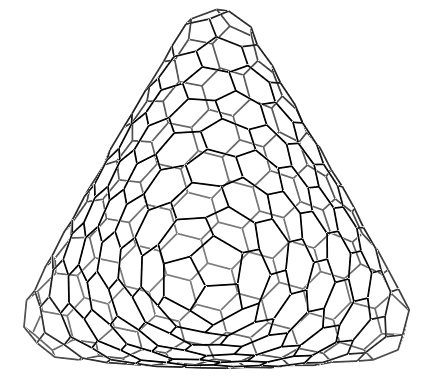
\includegraphics[width=0.4\textwidth]{C380.png}
	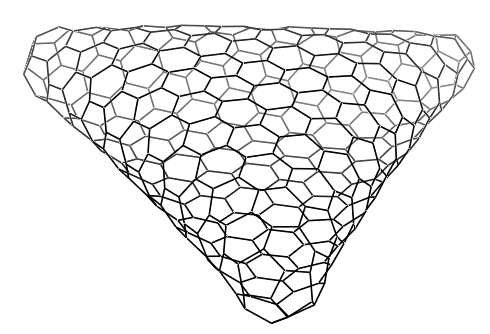
\includegraphics[width=0.5\textwidth]{C384.png}
    \caption{Optimized Wu force-field structures of \C{380} (left) and \C{384} (right), the first fullerenes with no ring spiral.}
	\label{pic:C380andC384}
 \end{figure}

Information from subroutine \funname{RingC} can be used to perform Stone-Wales transformations \cite{Stone86}
(subroutine \funname{StoneWalesTrans}), Endo-Kroto 2-vertex insertions \cite{Endo92} (subroutine \funname{EndoKrotoTrans}),
Yoshida-Fowler 4-vertex ($D_{3h}$ 6555) (subroutine \funname{YoshidaFowler4}) and 6-vertex ($D_{3h}$ 666555)
insertions (subroutine \funname{YoshidaFowler6}) \cite{Yoshida97a}, or a Brinkmann-Fowler 6-vertex (6-55-55) insertion 
(subroutine \funname{BrinkmannFowler}) \cite{BrinkmannFowler03}, see for example input files \textit{CCc50EK.inp, GEOMc60SW.inp, CCc80YF.inp}.
The vertex-insertion nomenclature introduced by Brinkmann and Fowler \cite{BrinkmannFowler03} defines these insertions uniquely:\\
Endo-Kroto: 2 pentagon G2.12.1.1 ($n_v$=12) $\rightarrow$ G2.12.1.2 ($n_v$=14);\\ 
Yoshida-Fowler 4 vertex insertion: 3 pentagon G3.15.31.1 ($n_v$=15) $\rightarrow$ G3.17.3.2 ($n_v$=19);\\
Yoshida-Fowler 6 vertex insertion: 3 pentagon G3.15.4.1 ($n_v$=19) $\rightarrow$ G3.15.4.2 ($n_v$=21) 
followed by G3.15.3.1 ($n_v$=15) $\rightarrow$ G3.15.3.2 ($n_v$=19);\\
Brinkmann-Fowler 6-vertex insertion: 4 pentagon G4.14.2.1 ($n_v$=16) $\rightarrow$ G4.14.2.2 ($n_v$=22).\\
Non-spiral fullerenes such as  \C{380} or  \C{384} can be constructed with such vertex insertion methods, see input files \filename{RSPIc380.inp} 
and \filename{RSPIc384.inp}. The two structures obtained from a force-field optimization are shown in Figure \ref{pic:C380andC384} using program PYMOL \cite{Pymol}.

Subroutine \funname{SpiralSearch} uses the ring-spiral algorithm of Fowler and Manolopoulos \cite{Atlas}
for the search of a ring spiral if, for the input, cartesian coordinates or vertex connections (adjacencies) were chosen, or if the
initial fullerene structure was modified. It produces the canonical ring-spiral pentagon indices
if the fullerene contains a face spiral, and fails if it does not (as for the two examples shown in 
Figure \ref{pic:C380andC384}). Note that considerable improvements were made to optimize the ring spiral search algorithm, and if 
\paramname{ispsearch}=2 is chosen it counts all possible ring spirals (this is computationally more expensive). 
The number of spirals in the output agree with the examples given by Yoshida and Fowler.\cite{Yoshida97a} 
A generalized ring-spiral algorithm has been implemented, and if the search for a canonical ring spiral algorithm fails, RSPIs are produced with additional jumps.


%Volume and surface area, minimum covering sphere
\subsection{Volume $V$ and surface area $A$, minimum covering sphere, \\ minimum distance sphere and maximum inner sphere}
The volume and surface area of the fullerene are calculated in Subroutine \funname{Volume}. This is done by\\
1) The convex hull.\\
2) The normal vector algorithm resulting in the exact volume of the polyhedron (identical to convex hull if polyhedron is convex).\\
3) The tesselation into trigonal pyramids from the barycenter by summing over all tetrahedrons spanned
by the three vectors (identical to algorithm 1 and 2 if the polyhedron is convex).  A sum over all
tetrahedrons spanned by the three vectors CM-CR (center(mass)-center(ring): barycenter of fullerene to the ring center),
CM-CA1 (barycenter of fullerene to atom~1 in ring), and CM-CA2 (barycenter of fullerene  to atom~2 in ring) is calculated.
There are 5 such tetrahedrons in a pentagon and 6 in a hexagon.  The barycenter CM has been set to the origin in a previous step.

In a similar way the surface area $A$ is obtained by summing over all triangles from the ring center to
neighbouring vertices in the ring. $I_h$-\C{20} and $I_h$-\C{60} coordinates can be constructed easily
using basic geometry. For these, the volume and surface areas are known analytically.

The \textit{isoperimetric quotient} (IPQ) is defined as
\begin{equation}
 q_{\textrm{IPQ}} =36\pi \frac{V^{2} }{A^{3}}\quad\text{with}\quad q_{\textrm{IPQ}}\in [0,1]
 \label{IPQ}
 \end{equation}
which for an ideal sphere is trivially $q_{\textrm{IPQ}}=1$, and for zero volume $q_{\textrm{IPQ}}=0$. For \C{20} 
and \C{60} with equal bond lengths we get
\begin{equation}
\label{IPQC20}
q_{\textrm{IPQ}} (\C{20}) =0.75470 
\end{equation} 
\begin{equation}
\label{IPQC60}
q_{\textrm{IPQ}} (\C{60}) =0.90317 
\end{equation} 

 We can now define the deviation from a sphere (in \%) by
\begin{equation} 
D_{\textrm{IPQ}} =100\left(1-q_{\textrm{IPQ}} \right) 
\end{equation}

The program also calculates the \textit{sphericity parameter} of Diaz-Tendero \cite{Diaz},
\begin{equation}
\label{Diaz}
q_{\textrm{SP}} = \sqrt{(a-b)^2+(a-c)^2+(b-c)^2}/A 
\end{equation}
where $a \ge b \ge c$ are the rotational constants. Note that we deviate from the original definition by dividing 
the square-root by the rotational constant $A$. Further, the \textit{asymmetry parameter} of Fowler is printed,
\begin{equation}
\label{Diaz}
q_{\textrm{AP}} = \sum_{i=1}^{n_v}  \frac{(r_i-r_{av})^2}{r_{av}^2}
\end{equation}
where $r_i$ is the radial distance of atom $i$ from the barycenter and $r_{av}$ is the average distance \cite{Fowler2000}.

Three routines follow to calculate the \textit{minimum covering sphere} (MCS) of a fullerene (Subroutine
\funname{MinCovSphere2}) using algorithm 2 of Yildirim \cite{Yildirim08}, \textit{minimum distance
sphere} (MDS) (Subroutine \funname{MinDistSphere}), and the \textit{maximum inner sphere} (MIS) (Subroutine \funname{MaxInSphere}).
The MCS is defined as follows:
Let $S = \vec{p}_i$ be the set of $n$ points ($i=1,\ldots ,n$) in $m$-dimensional Euclidean space, 
$\mathbb{R}^m$. The MCS of this set, MCS($S$), is a sphere of smallest radius $R_{MCS}$ that encloses the set of points $S$,
and can be expressed as follows,
\begin{equation}
	\label{eq:MCS}
	\min\limits_{\vec{c}_{\mathrm{MCS}} } \max\limits_i \left\| \vec{p}_i -\vec{c}_{\mathrm{MCS}} \right\|  
\end{equation} 
where $\|\cdot\| $ denotes the Euclidean norm and $\vec{c}_{\mathrm{MCS}}$ is the center of the MCS. The MCS
is uniquely defined and can be expressed as a convex combination of at most 
($m+1$) points, hence our algorithm stops when 4~points are left over in the iteration process of the algorithm.
The spherical central cover SCC is not the minimum covering sphere MCS
(except for example if all distances from the barycenter CM are the same as in the
ideal capped icosahedron). The spherical central cover is taken from the
CM point with radius $R_{\mathrm{max}}$ (longest distance to one vertex).  We changed the first
condition in Yildirim's algorithm by choosing $R_{\mathrm{max}}$ as the furthest point from CM.
In the final statistics there should be 0 points outside the sphere and at least 1 point on the sphere.
We can now introduce the definition for the MCS distortion parameter $D_{MCS}$ (in \% of $r_{\mathrm{min}}$),
\begin{equation} \label{eq:DMCS}
D_{\mathrm{MCS}} =\frac{100}{n_vr_\mathrm{min}} \sum_{i=1}^{n_v} \left(R_{\mathrm{MCS}} - \|\vec{p}_i - \vec{c}_{\mathrm{MCS}}\|\right)
\end{equation} 

At the end, the Van der Waals radius of carbon (1.415\,\AA) is added to the radius of the MCS
(input coordinates for this need to be in \AA{} otherwise you are required to change the program),
and the volume of an ideal fcc solid is calculated. The Van der Waals radius is chosen such that
for \C{60} the solid-state results of Heiney et al. \cite{Heiney91} are reproduced.
In the case of nonplanar pentagons or hexagons there is no unique definition for the volume of a fullerene,
except for the convex hull. There is no reason, however, why any other definition should be preferred
over the exact volume algorithm employed in this program.

The MCS is biased for the case that few atoms stick out on the surface of a fullerene,
and the minimum distance sphere (MDS) may be more appropriate for a measure from spherical distortion,
\begin{equation} 
\min\limits_{c_\mathrm{MDS} \in CH(S)} \frac{1}{n_v} \sum _{i} \left|R_\mathrm{MDS} -\left\| \vec{p}_{i}-\vec{c}_\mathrm{MDS} \right\| \right|  
\end{equation}

with the MDS radius
\begin{equation} 
	R_{\mathrm{MDS}} =\frac{1}{n_v} \sum _{i}\left\| \vec{p}_{i} -\vec{c}_{\mathrm{MDS}} \right\|   
	\label{eq:RMDS}
\end{equation} 

The restriction of $\vec{c}_{\mathrm{MDS}}$ to be inside the convex hull is necessary as $\vec{c}_{\mathrm{MDS}}$ may move
out of the fullerene structure in the optimization procedure.  In general we have $\vec{c}_{\mathrm{MDS}}\ne\vec{c}_{\mathrm{MCP}}$
except for the case that all points lie on the MCS. The MDS may however not be uniquely defined, as there could be many 
(even degenerate) local minima, but for most cases (i.e. ``spherical'' fullerenes) it works just fine.  
This gives a better definition for the distortion
parameter compared to $D_{\mathrm{MCS}}$, as it is not biased to a few points lying outside or inside the fullerene surface.
Hence, analogous to the MCS we define a measure for distortion from spherical symmetry through the MDS,
\begin{equation}
  \label{eq:DMDS}
  D_{\mathrm{MDS}} = \frac{100}{n_v r_{\mathrm{min}}} \sum_{i=1}^N \left|R_{\mathrm{MDS}} - \|\vec{p}_i - \vec{c}_{\mathrm{MDS}}\| \right|
\end{equation}

The maximum inner sphere (MIS) is important to estimate if there is enough space inside the fullerene cage for endohedral atoms or molecules. It is
defined as
\begin{equation}
	R_{\mathrm{MIS}} = \max\limits_{c_{\mathrm{MIS}} \in \mathrm{CH}(S)} \min\limits_{i} \left\| \vec{p}_{i} -\vec{c}_{\mathrm{MIS}} \right\|  
	\label{MES} 
\end{equation}

For ideal \C{60} ($I_h$ symmetry) MCS, MDS and MIS are all identical. Note that the MIS may not be uniquely defined. For example, for nanotubes
there may be degenerate solution with different $\vec{c}_{\mathrm{MDS}}$ along the main axis of the nanotube.
For the MIS the radius and volume is printed  with the Van der Waals radius of carbon taken off $R_{\mathrm{MIS}}$. 

%2D fullerene graphs and Schlegel diagrams
\subsection{2D fullerene graphs and Schlegel diagrams}
Fullerenes can be nicely visualized by 2D fullerene graphs. They should be distance-transitive, distance-regular and 
symmetric. There are a number of different algorithms available trying to achieve this, and in subroutine \funname{Graph2D} $(X_i,Y_i) (i=1,\dots, n_v)$ 
coordinates for a 2D fullerene graph are created. Here we briefly describe the algorithms we recommend to use,
others are of perhaps of more historical interest. Note that for non-spherical fullerenes (like the famous non-spirable \C{380} (Figure  \ref{pic:C380andC384})
tetrahedron) it becomes very difficult to create a good Schlegel projection, and in such cases the projection of vertices to the minimum
covering sphere is recommended before these algorithms are used (see input). The subroutine produces a latex file with the fullerene graph included.

1) In the perspective Schlegel projection (PSP), the 3D graph is rotated such that a selected vertex, edge of ring 
(commonly the barycenter of a polygon is chosen) is located at top of the $z$-axis at some distance below the projection point $P$, 
with the $z$-axis going (not necessarily) through the barycenter of the fullerene. If no choice is given in the input, the point $(0,0,z_{\mathrm{max}})$ 
is chosen with $z_{\mathrm{max}}$ being the point with maximum $z$-value from the original input coordinates of the vertices. 
Vertices and ring barycenters are then sorted in descending order according to their $z$-values.
The Schlegel projection then yields the projected $(X_i,Y_i)$ coordinates by projecting vertices and ring centers 
down on a plane below the fullerene.  The edges between the vertices are already known such that the fullerene graph can be drawn. 
This is shown in Figure \ref{pic:Schlegel}.

%Figure 4
 \begin{figure}[htbp]
   	\centering
  	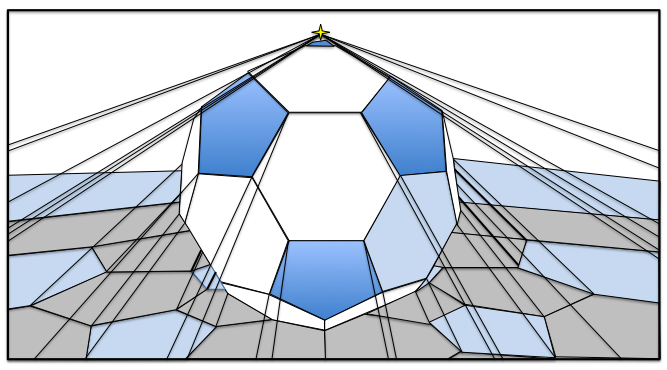
\includegraphics[width=0.5\textwidth]{Schlegel.png}
    \caption{Perspective Schlegel projection for \C{60}.}
	\label{pic:Schlegel}
 \end{figure}

2) In the cone Schlegel projection (CSP) the vertices are projected out on an enveloping cone and then down on a plane below the fullerene. 
The barycenter of the last ring closest to the projection plane should be at the bottom of the fullerene. The barycenter of the circumfencing
ring will not be projected out (this center may be ignored in the drawing). A scaling factor could be applied (1.2 used in the program)
for the outer points in the 2D graph in order to avoid edge crossings.
       
At the end a rough plot of the fullerene graph is produced. This is suitable for fullerenes up to about \C{100}, beyond that
it becomes too crowded and the latex file produced contains a better graph. Nevertheless, it serves for a first rough picture. 
Furthermore, for large fullerenes it becomes critical to correctly set the projection point or point of the cone.
If, for example the projection point is too far away from the fullerene, edges in the 2D graph may cross.

3) Tutte 2D embedding with linear scaling (2D-TE-LS). Here the Tutte algorithm is used \cite{Tutte}
but the resulting overcrowding of small polygons near the center of the graph is remedied
by a linear scaling procedure
\begin{equation}
	\label{GrindEQ__16_} 
	\lambda_i = 1+\frac{f(r_\mathrm{min} - r_i)}{r_\mathrm{min}}
\end{equation}
applying a linear scaling factor $\lambda_i$ to all vertices $v_i$ ($i=5(6),\dots , n_v$), where $f$
is a parameter to be determined, $r_{\mathrm{min}}$ is the smallest distance to the vertices of the peripheral
taken from the barycenter $P$ of the innermost ring (or alternatively the barycenter of the 2D convex hull), 
and $r_i$ is the distance from that point $P$ to the vertex $v_i$.

4) Pisanski-Plestenjak-Graovac embedding algorithm (PPGA) \cite{pisanski95}. This is one of the more successful algorithms developed by 
Pisanski, Plestenjak and Graovac in conjunction with a simulated annealing procedure for better visualization of graphs, 
which is an improvement over usual spring embedders. Here the potential between adjacent vertices is modeled by
\begin{equation} 
\label{eq:Eppg} 
E_{\mathrm{PPG}} =\sum_{i<j}^{\mathrm{ord}(G)} A_{ij}  r_{ij}^{2} \exp \left(\alpha \frac{2d_{\mathrm{max}} -d_{iP} -d_{jP} }{d_{\mathrm{max}} } \right) 
\end{equation} 
where $A_{ij}$ is the adjacency matrix, $r_{ij}$ the distance between vertex $i$ and $j$, and $\alpha$ a
parameter to be determined. The distances in eq.\eqref{eq:Eppg} are defined through the topological
distance matrix $D$,
\begin{equation}
	\label{GrindEQ__20_}
  	d_{\mathrm{max}} = \max_{j,j_P}\left\{ D_{ij_P} \right\}\quad\text{and}\quad d_{ip} = \min_{j_P}\left\{ D_{ij_P} \right\}
\end{equation}
where  $j_P$ is the vertex number belonging to the (5 or 6) peripheral vertices.  Instead of a
simulated annealing algorithm we start with a Tutte 2D graph and perform a minimization procedure for $E_{\mathrm{PPG}}$.

For other 2D graph embedding methods implemented as shown in Figure \ref{pic:ManySchlegel} see the following input section.

\vspace{1cm}       
%Figure 7
 \begin{figure}[htbp]
	\centering
  		 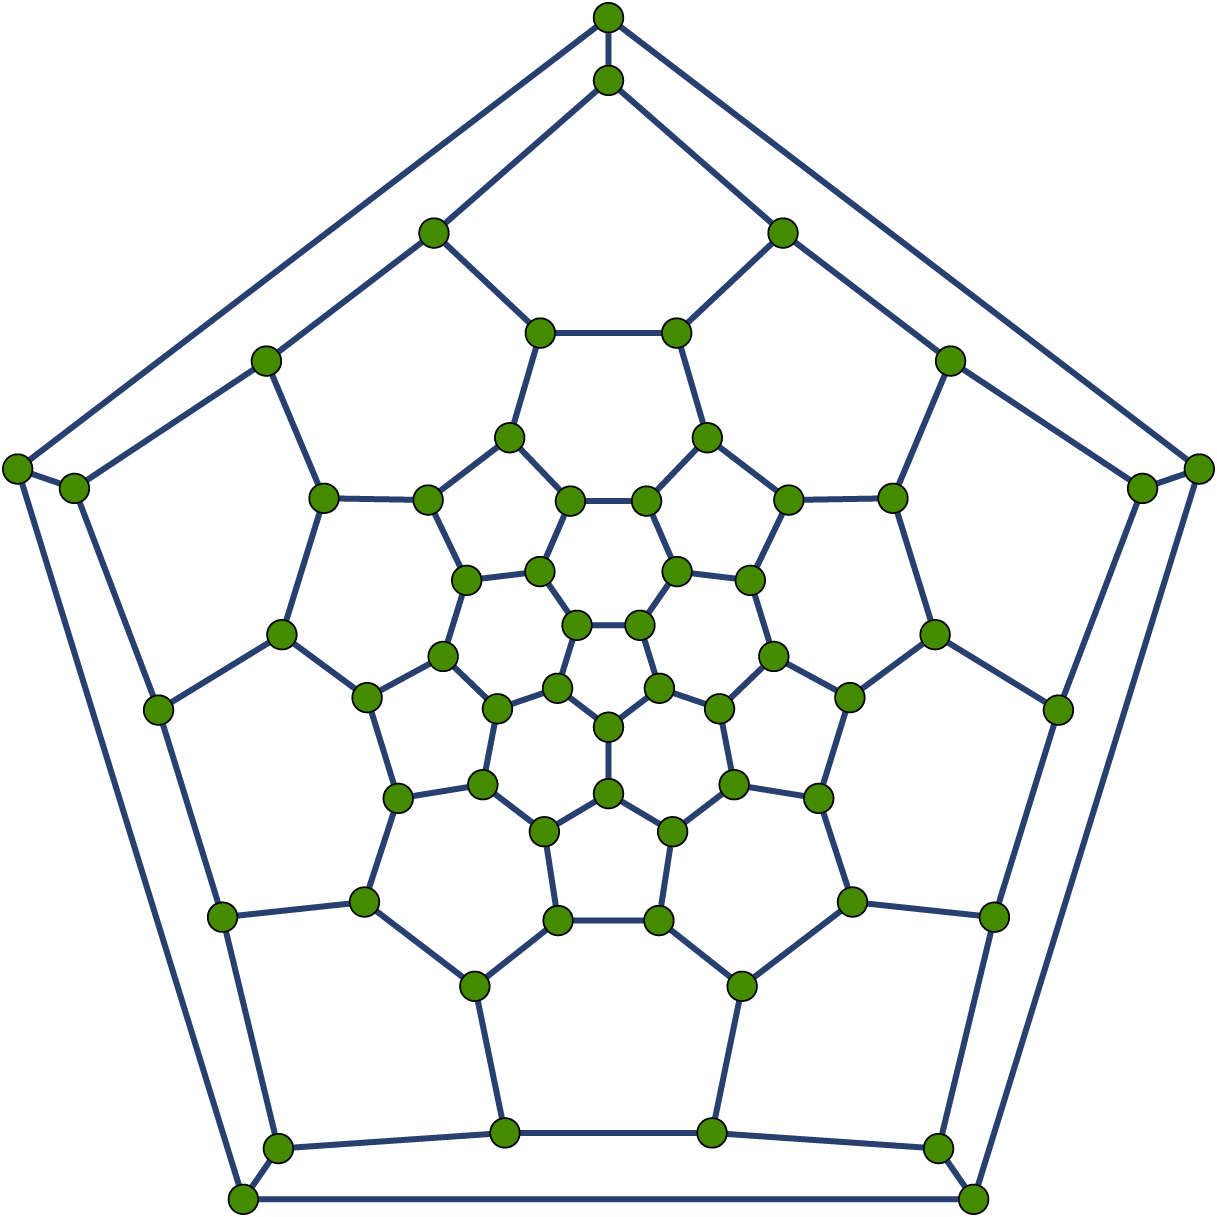
\includegraphics[width=0.225\textwidth]{Graph1.png}
		 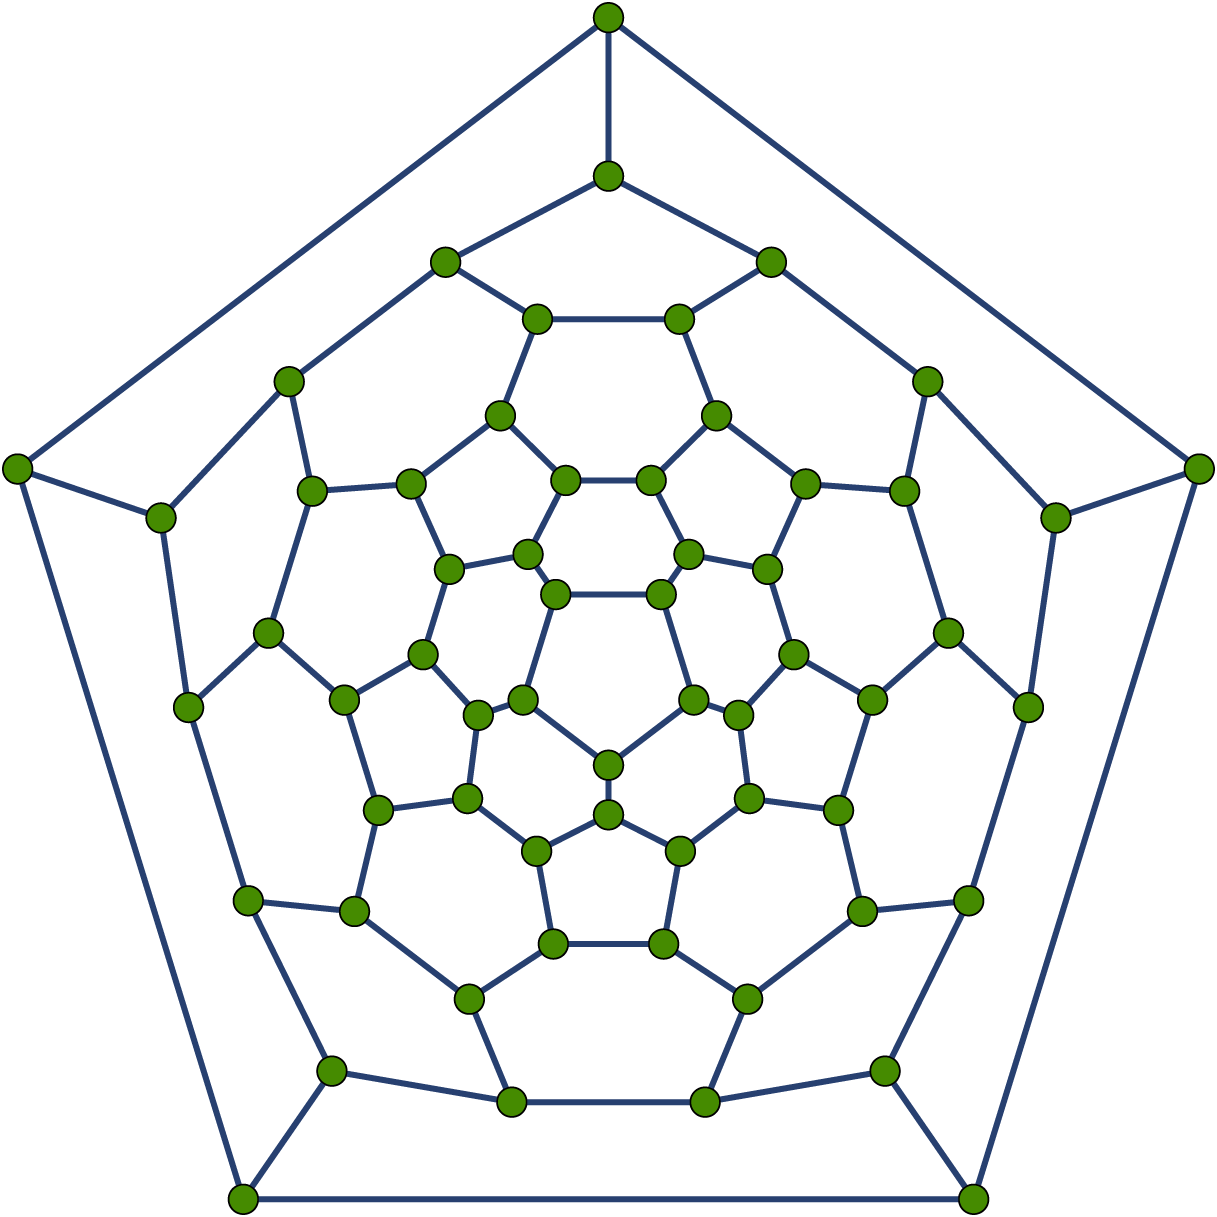
\includegraphics[width=0.225\textwidth]{Graph2.png}
		 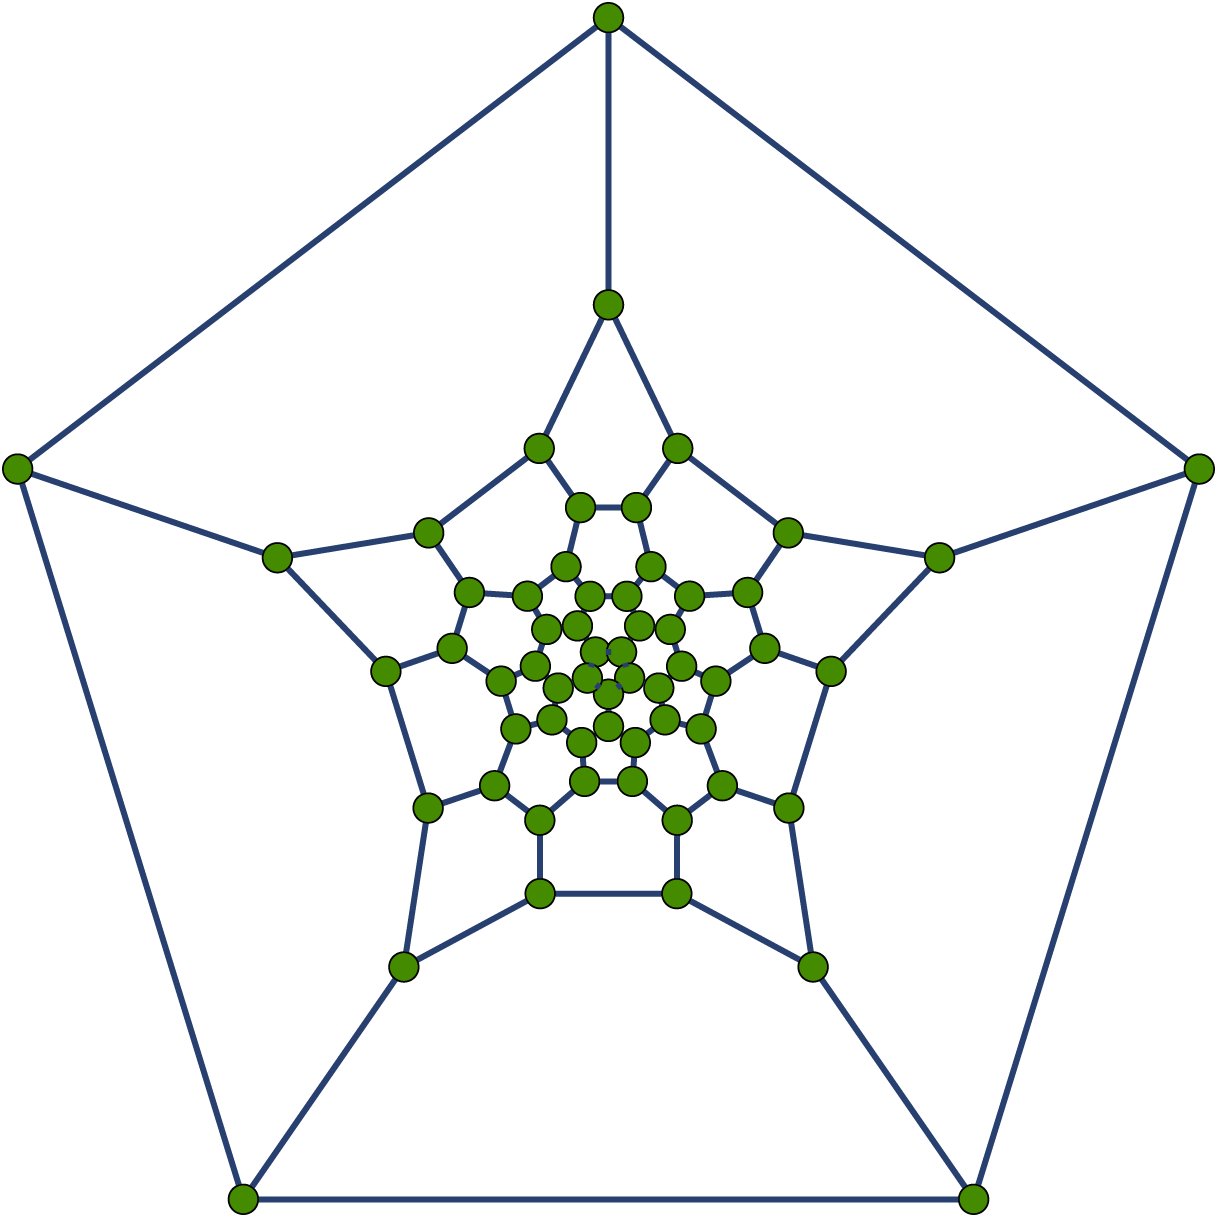
\includegraphics[width=0.225\textwidth]{Graph3.png}
		 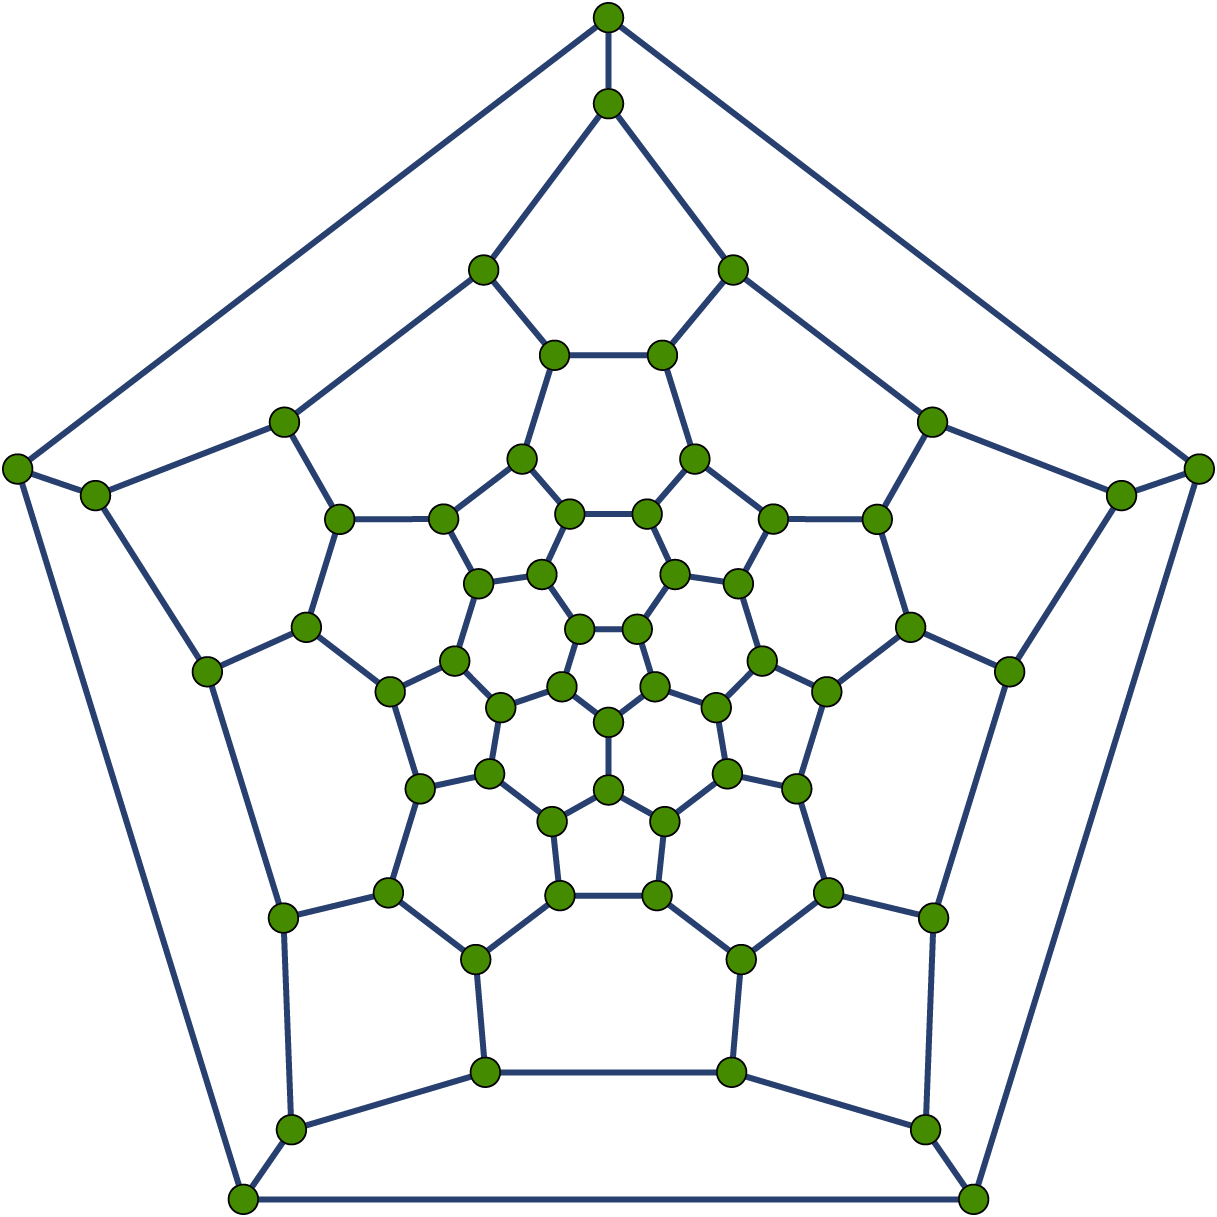
\includegraphics[width=0.225\textwidth]{Graph4.png}
		 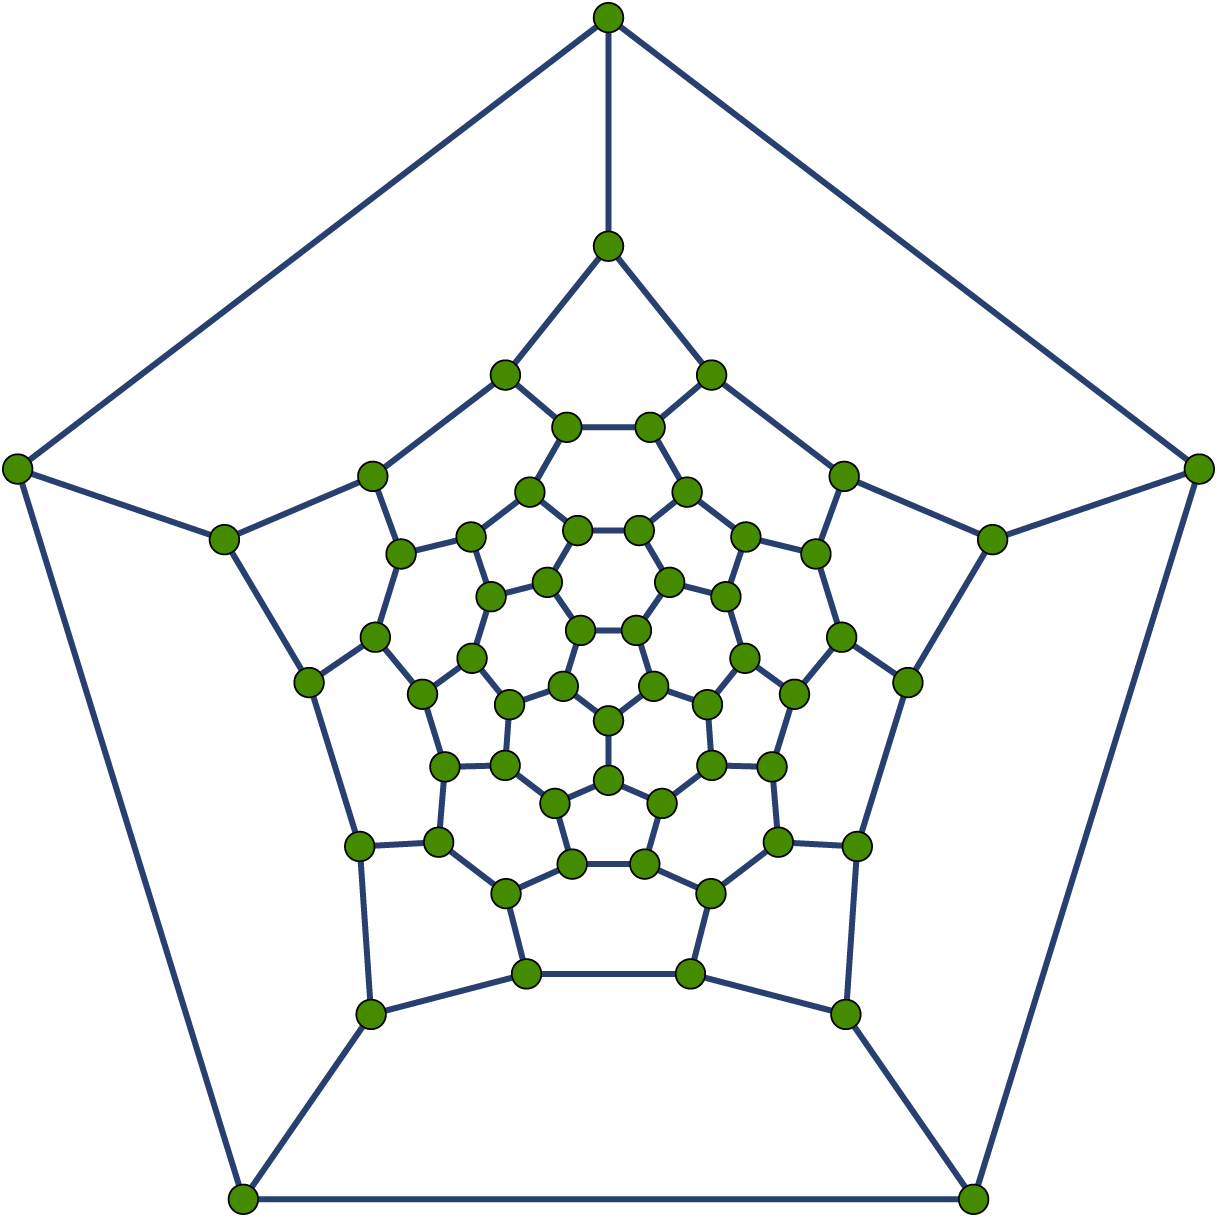
\includegraphics[width=0.225\textwidth]{Graph5.png}
		 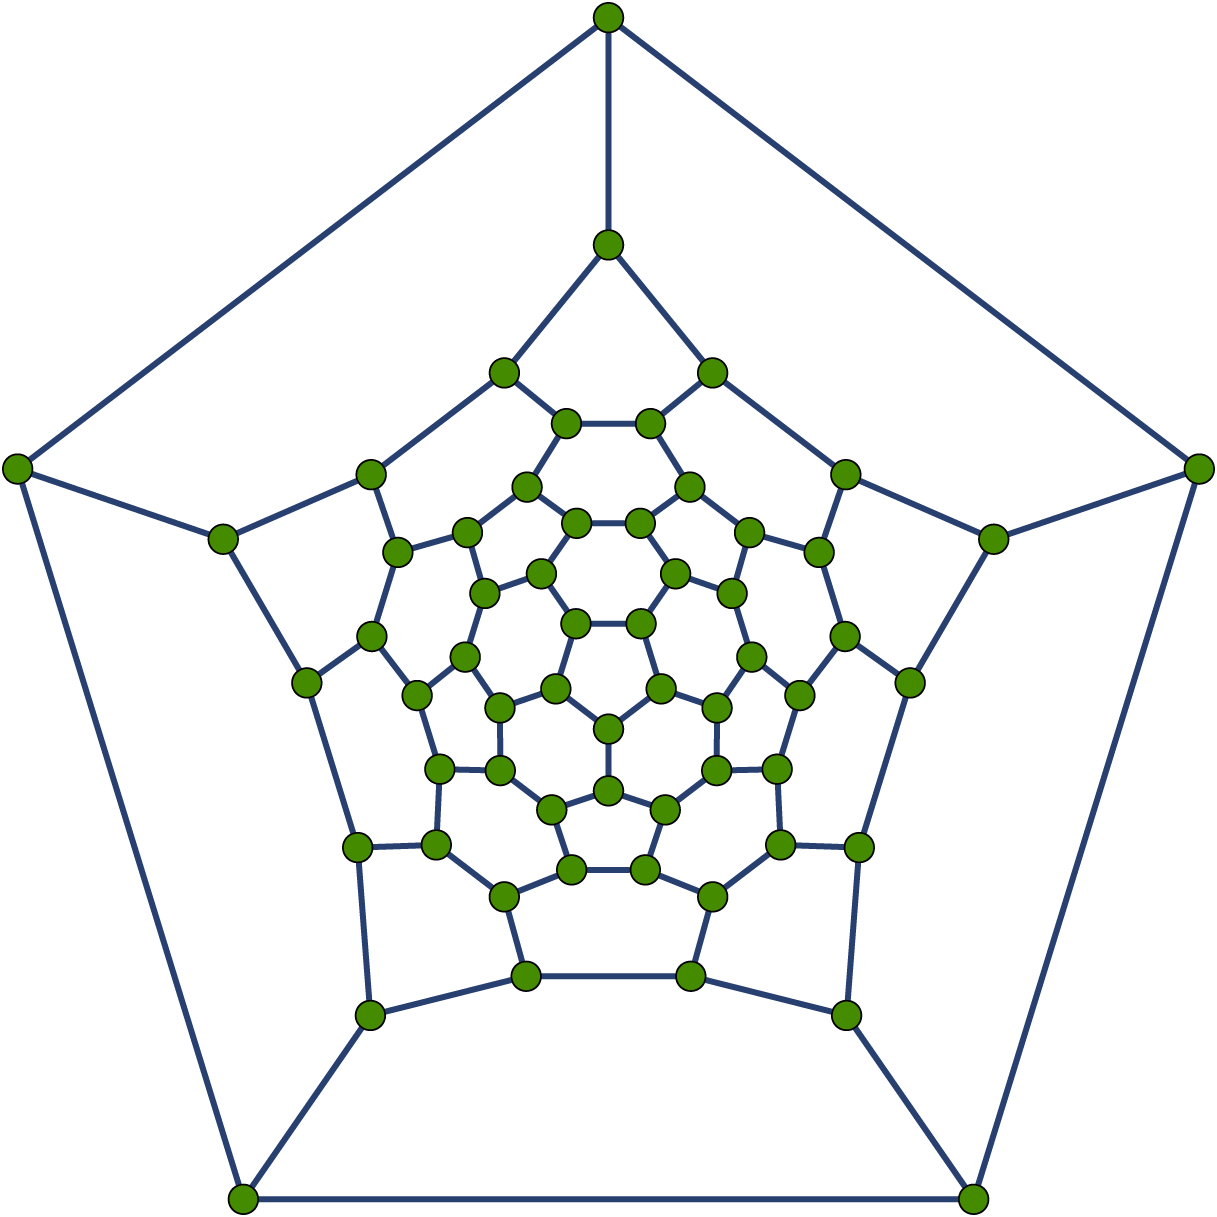
\includegraphics[width=0.225\textwidth]{Graph6.png}
		 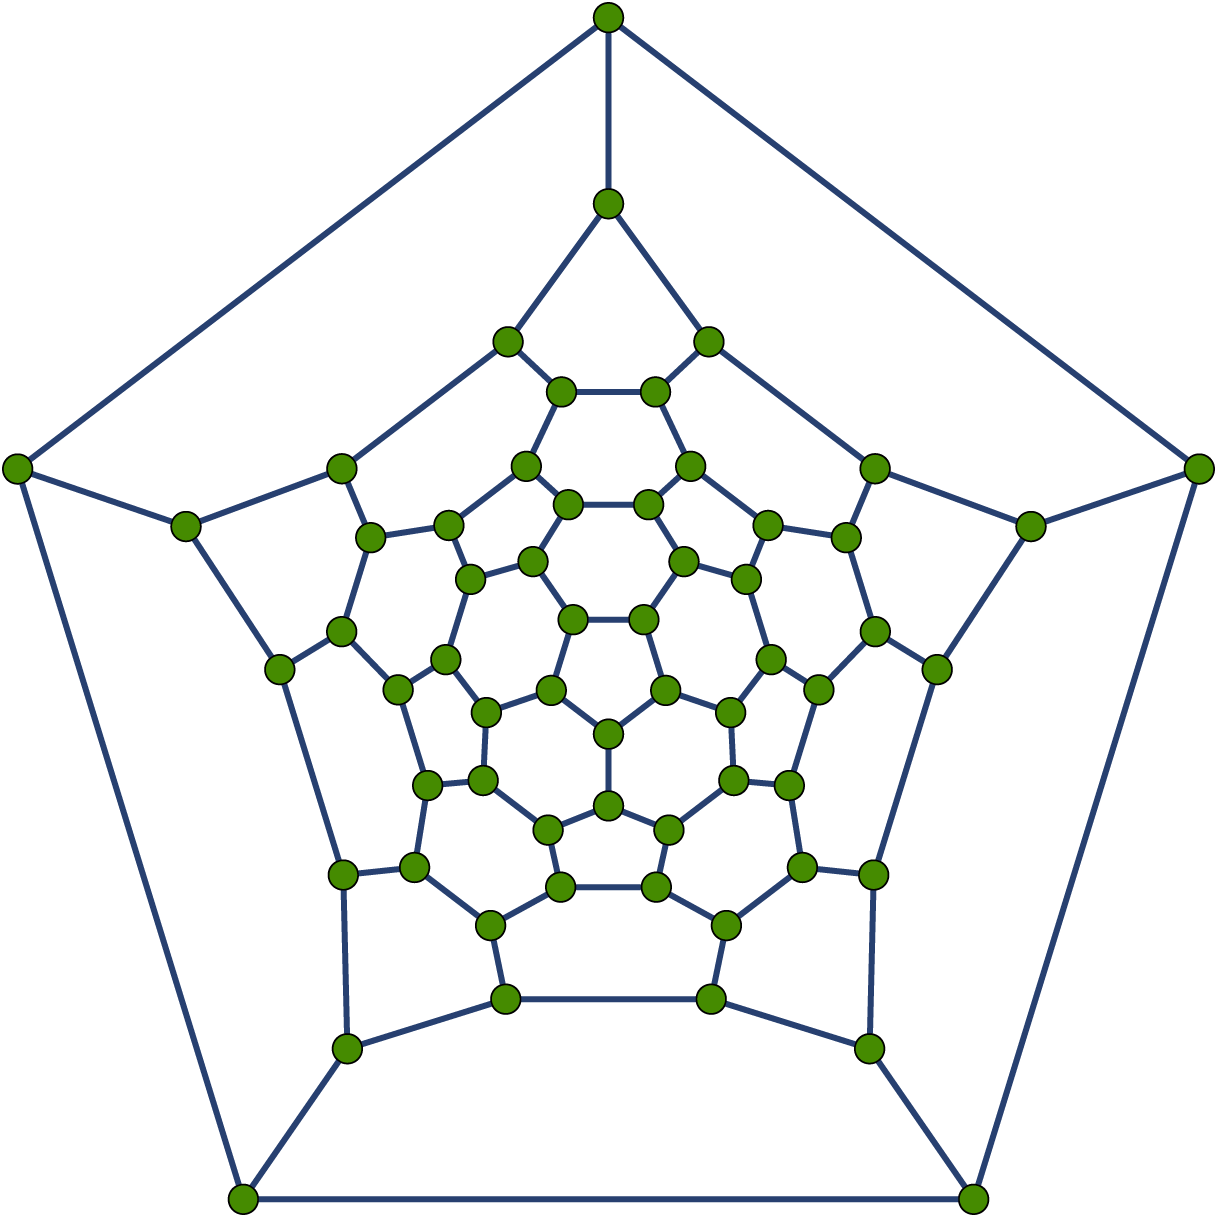
\includegraphics[width=0.225\textwidth]{Graph7.png}
		 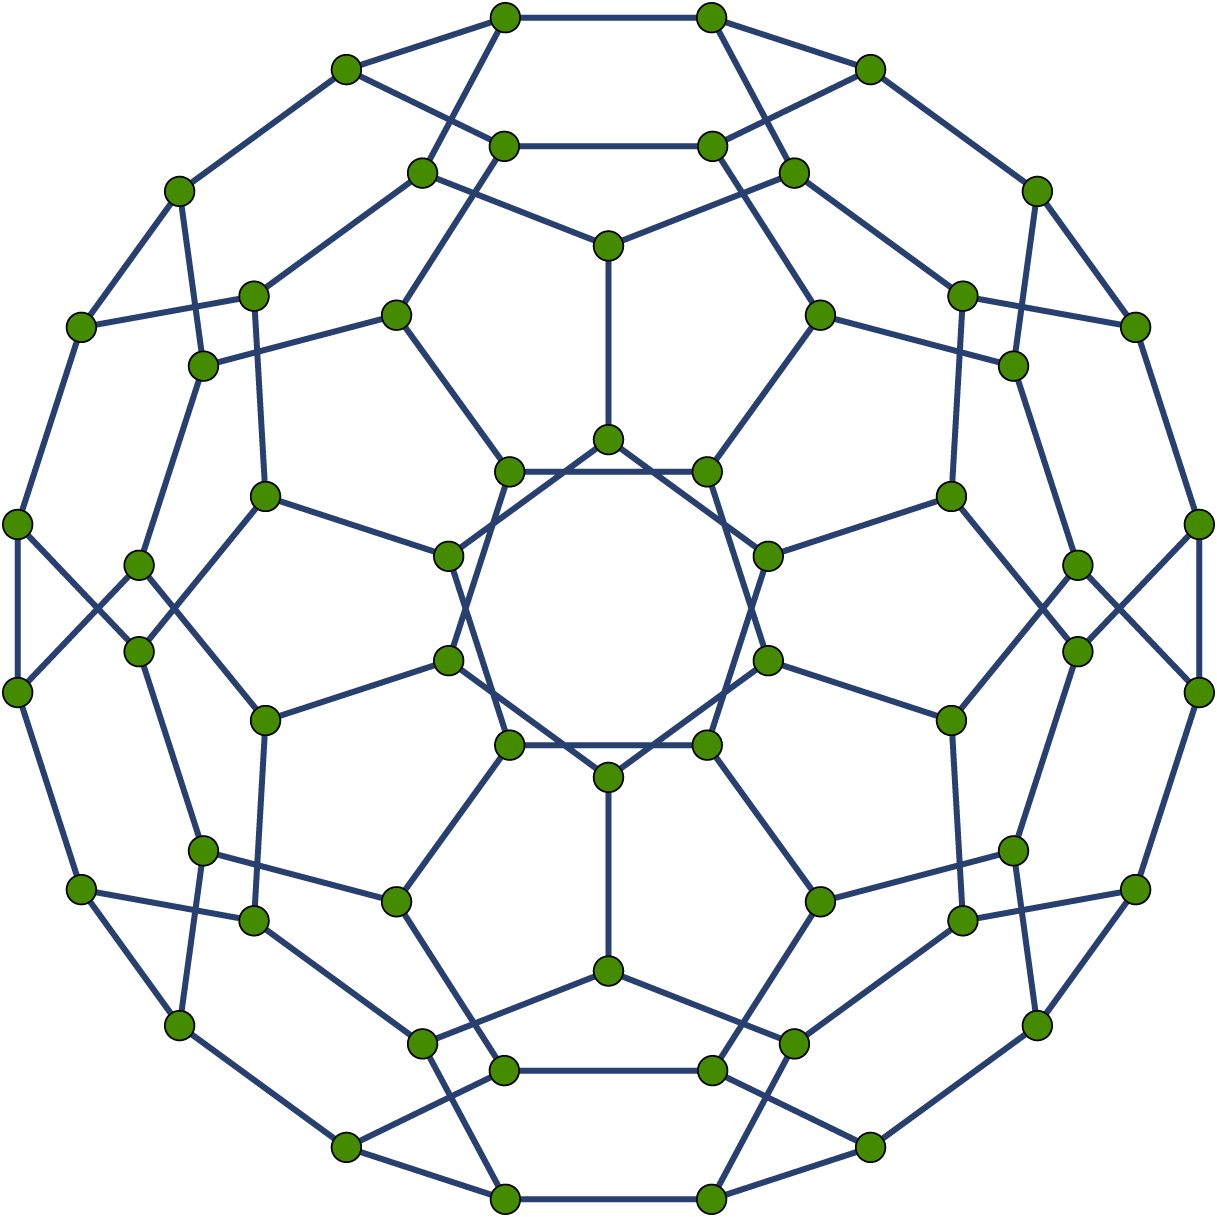
\includegraphics[width=0.225\textwidth]{Graph8.png}
     \caption{From the left to right: 2D fullerene structures created using \paramname{ISchlegel}=1 to 8 described in the input section.}
     \label{pic:ManySchlegel}
 \end{figure}

\clearpage
%Input description
\section{Input description}

Input and output files are in the directories \textit{input}  and   \textit{output}  respectively. \textit{Program Fullerene} has been tested 
for many fullerenes found in the following input files:\\
\begin{enumerate}
\item[1:] All files starting with \filename{CC} have cartesian coordinates for input, for example for
\C{20} (\filename{CCc20.inp}), \C{24} (\filename{CCc24.inp}), \C{60} (\filename{CCc60.inp}), or \C{540} (\filename{CCc540.inp}).
\item[2:] All files starting with \filename{GEOM} use basic geometry to construct \C{20} or \C{60}, e.g. \filename{GEOMc60.inp} or \filename{GEOMc60exp.inp}.
\item[3:] All files starting with \filename{EDGE} have vertex connectivities as input, e.g. \filename{EDGEc20.inp}.
\item[4:] All files starting with \filename{RSPI} have the ring-spiral pentagon indices as input, e.g. \filename{RSPIc20.inp} or \filename{RSPIc60NT.inp}
including and the non-spirable fullerenes \C{380} (\filename{RSPIc380.inp}) and \C{384} (\filename{RSPIc384.inp}).
\item[5:] All files starting with \filename{ISOMER} produces an isomer list, e.g. \filename{ISOMERc92.inp}.
\item[6:] All files starting with \filename{GC} uses the Goldberg-Coxeter transform of \C{20}, e.g. \filename{GCc720Halma.inp}.
\item[7:] All files starting with \filename{READ} uses an external \filename{.xyz} file to read in in cartesian coordinates, e.g. \filename{READxyz.inp}.
\end{enumerate}
Many more examples can be found. The cartesian coordinates used in the input files are mostly singlet electronic state 
B3LYP aug-cc-pVDZ optimized up to \C{60}, cc-pVDZ up to \C{180}, and 6-31G for the rest. 
For some of the fullerenes listed, the singlet state chosen may not be the electronic ground state.
Many definitions depend on the use of {\AA}ngstr{\o}ms for distances, so please use this unit throughout. 
A typical input is in \textit{Namelist format}, or if additional data are required in \textit{free format}, and reads like this:
\begin{verbatim}
C80  Using FM algorithm to produce coordinates for C80 nanotube, \\
input file: \filename{RSPIc80NT.inp}
&General NA=80 / 
&Coord ICart=2, IV2=4, IV3=5 , rspi=1, 2, 3, 4, 5, 6, 37, 38, 39, 40, 41, 42 /
&FFChoice Iopt=1 / 
&FFParameters / 
&Hamilton IHam=1 / 
&Isomers IPR=1 / 
&Graph ISchlegel=2, ISO1=2, ISO2=4, ISO3=5 / 
\end{verbatim}
The first line is a text line, the second \&General is a general
command line in \textit{namelist format} containing many useful flags,
the third \paramname{\&Coord} line tells the program how the
coordinates are created, the next two lines \paramname{\&FFChoice}
and \paramname{\&FFParameters} are specifications for the force field
to be used (none in this case), line 5 (\paramname{\&Hamilton})
concerns the Hamiltonian cycles, line 6 (\&Isomers) is for an isomer list
to be created, and line 7 (\paramname{\&Graph}) for the 2D fullerene
graph (Schlegel diagram). The last line in the input is for other input required, e.g.
the indices for vertex insertions.

In the following, the input in the required sequence is described in detail (either Namelist or in Free Format):

\subsection{Comment line} 
A comment line of of max. 132 characters. You can have as many comment lines as you want, so long as they are 132 characters or less: 
every line until the first namelist line is interpreted as a comment.

%---General---
\subsection{\&General line}
Namelist line that contains the main flags for the program. 

\paragraph{List of options:}\  \paramname{NA, IP, ixyz, ichk, nohueckel, loop, ipsphere, nosort, ispsearch, novolume, TolR, R5, R6, filenamedb, filename, ndbconvert, IPMC}.
\paragraph{Option description:}
\begin{description}
\item[{NA}]   Number of atoms (vertices) $N_A$ (Default: 60)
\item[{IP}]  If set to 1, verbose output is be produced, i.e. the full distance matrix, all Hamiltonian cycles 
  and all ring connections up to three rings (Default: 0).
\item[{iwext}] Flag for producing input file for \program{CYLview}, \program{Avogadro} or other plotting programs in standard formats (Default: 0)
  Default name for the external file is \filename{Fullerene-3D} with the appropriate ending. Otherwise \paramname{filename}='filename' needs to be specified (max. 50 characters).
  Note that if the routine which writes out \filename{.xyz}, \filename{.cc1} or \filename{.mol2} files is used more than once, for example through the \paramname{nloop} parameter,
  a number is added after the string "-3D" in order to not cause conflict with previous files. Note that the filenames will have a number attached to it when written out,
  i.e. \filename{filename-3D.xyz}, \filename{filename-3D2.xyz} etc. (the case \paramname{nloop}=1 is omitted in the name)\\
  If \paramname{iwext} = 1: Write out external \filename{.xyz}  file named \filename{filename-3D.xyz} for further input.\\
  If \paramname{iwext} = 2: Write out external \filename{.cc1}  file named \filename{filename-3D.cc1} for further input.\\
  If \paramname{iwext} = 3: Write out external \filename{.mol2} file named \filename{filename-3D.mol2} for further input.\\
\item[{irext}] Flag for reading external input file which contains cartesian coordinates or connectivities (Default: 0). Note this makes the input of \paramname{ICart} obsolete if set non-zero.
  If \paramname{irext} = 1: Read \filename{.xyz} from file specified by \paramname{filename}. The final name is chosen as \filename{filename.xyz} (Default: \filename{Fullerene.xyz}). 
  Another \filename{.xyz} file is also produced and named \filename{filename-3D.xyz} if \paramname{iwext} = 1 is specified.\\
  If \paramname{irext} = 2: Read \filename{.cc1} from file specified by \paramname{filename}. The final name is chosen as \filename{filename.cc1} (Default: \filename{Fullerene.cc1}). 
  Another \filename{.cc1} file is also produced and named \filename{filename-3D.cc1} if \paramname{iwext} = 2 is specified.
  .cc1 files contain information about vertex connections. Programs like PYMOL can read such files. This is useful for reading for example \filename{.cc1} files produced 
  by M. Yoshida \cite{Yoshida}, which has been added to our database.\\
  If \paramname{irext} = 3: Read \filename{.mol2} from file specified by \paramname{filename}. The final name is chosen as \filename{filename.mol2} (Default: \filename{Fullerene.mol2}). 
  Another \filename{.mol2} file is also produced and named \filename{filename-3D.mol2} if \paramname{iwext} = 3 is specified.
  The file is in standard Tripos format.\\
\item[{nohueckel}]  If \paramname{nohueckel} = 1 diagonalization of H\"uckel matrix is avoided which is of order $\mathcal{O}(n^3)$ (recommended for large matrices over size 5000) (Default: 0).
\item[{loop}] 
  If \paramname{loop} = 1: New input required (compound job), i.e. program does not stop at the end but loops back to the beginning (Default: 0). 
  This is important if one takes an initial structure and subjects it to further transformations, for example in subsequent Stone-Wales or
  Goldberg-Coxeter transformations. You might use this option to read from a .xyz file created in the previous run.\\
  If \paramname{loop} = 2: Same as above but if \paramname{ICart} specified correctly, it takes pentagon indices from a previous run.
\item[{ipsphere}] 
  Project all vertices onto the minimum covering sphere (MCS), useful for drawing 2D fullerene graphs (Default: 0).
  \begin{enumerate}
  \item[1:] Project vertices onto MCS.
  \item[2:] In addition, write MCS to the .xyz-file \filename{filename-3DMCS.xyz}.
  \item[3:] In addition, write MCS to the .cc1-file \filename{filename-3DMCS.cc1}.
  \end{enumerate}
\item[{nosort}] If \paramname{nosort} = 1, permutation of vertices for better $Z$-Matrix is suppressed (Default: 0).
\item[{IPMC}] If \paramname{IPMC} = 1, the number of perfect matchings are counted using the Pfaffian (Default: 0).
\item[{ispsearch}] If \paramname{ispsearch} = 0, search for the canonical ring spiral is avoided  (Default: 1). If \paramname{ispsearch} = 1, ring spiral search takes place
until it is successful. If \paramname{ispsearch} = 2, all spirals are counted (this is computationally expensive for very large fullerenes). 
\item[{novolume}] If \paramname{novolume} = 1, all parts for volume determination is avoided  (Default: 0).
\item[{TolR}] Tolerance in \% (Default: 33). Only change this parameter if the program cannot produce correctly the adjacency matrix. 
  This is only necessary for the cartesian coordinate input (\paramname{ICart}=1) and only fails if bond distances are unusually large or small. 
  Connectivities are found for atoms with distances between \paramname{R6} and $\paramname{R6}*(1+\paramname{TolR}/100)$. 
  If this parameter is set at a value too large, unwanted connectivities are produced resulting in smaller polygons. 
  This parameter should reflect the maximum deviation in distance from the smallest distance found.
\item[{filename}] 
    Prefix for for all external filenames created by the program. Limited to 50~characters. Default: \filename{Fullerene}.
\item[{filenameout}] 
    Prefix for for a database filename to be used as output for .xyz and .cc1 files if different from \filename{filename}. Limited to 50~characters, 
    Used for example to read from the Yoshida or House of Graph files with \filename{filename} in the directory \filename{database/Yoshida} or \filename{database/HOG}.
    and write .xyz-file out to another filename called \filename{filenameout}.
\item[{ndbconvert}] Programmers option to convert output from isomer routine into a more compact format.
\item[{imcs}] By setting \paramname{imcs}=1 only minimum covering sphere is calculated. This works only for \paramname{ICart}=1 (see next input section), however, in this case any cartesian coordinate input can be taken, i.e., any points in 3D space.
\item[{itop}] If \paramname{itop} = 1, after creating the adjacency matrix skips directly to the topological analysis. Good for very large fullerenes, e.g. Goldberg-Coxeter transforms. If \paramname{itop} = 2 in addition writes out the connectivity vector to external file \filename{ic3file} (formatted), which can be used as further input.
\end{description}


%---Coord---
\subsection{\&Coord line}

Input to create cartesian coordinates for the program (e.g. \verb|&Coord ICart=2, R6=1.42 /|).
\paragraph{List of options:}\ 

\paramname{ICart, rspi, jumps, IV1, IV2, IV3, isonum, leap, IGCtrans, kGC, lGC, ISW, KE, IYF, ISW, mirror, IPRC, R5, R6, ScaleRad, nanotube}

\paragraph{Option description:} 
\begin{description}
\item[{ICart}] Flag for the construction of the 3D structure (cartesian coordinates) (Default: 0). For more details see below.\\
If \paramname{ICart} = 1 then Cartesian Coordinate input is expected.\\
If \paramname{ICart} = 2, 3 then 12 pentagon indices are used for input using \paramname{rspi}.\\
If \paramname{ICart} = 4, 5 then Goldberg-Coxeter transformation of \C{20} is used, i.e. $GC_{k,l}(20)$ with $k \geq l$ and $k > 0$.\\
If \paramname{ICart} = 2 or 3 and \paramname{isonum} $\neq 0$, then pentagon indices are taken from the
isomer list contained in a database (see below).\\
If \paramname{ICart} = 6 or 7 input vertex connectivities (edges) directly. If \paramname{isonum} $\neq 0$,
then the isomer number from the isomer list contained in the ``House of Graphs'' database is taken. For the
vertex connectivities input as series of cards is required each with 4~integers: IV1, IC1, IC2, IC3,
i.e., 1~3~6~4 gives the following edges: 1-3, 1-6, and 1-4.  Zeros for IC2 and IC3 can be used, i.e. 1~3~6~0
gives 1-3 and 1-6, and 1~3~0~0 just gives 1-3 as an edge.  For the last card in the input stream, IV1 needs
to be set to zero. For an example see input file \filename{EDGEc20.inp}.  It is legal but not necessary to define edges twice.\\
If \paramname{ICart} = 8 or 9, general spiral input is required using  \paramname{rspi} and \paramname{jumps}.\\ 
If \paramname{ICart} = 10 A spiral search algorithm is used, see \paramname{isearch} keyword in \paramname{Isomer} section.

When importing graphs from the ``House of Graphs'' database, the isomers are numbered starting at~1 (Although,
internally we start counting at~0.).  There are two example files called \filename{DBc50HOG.inp} and \filename{DBc384HOG.inp}.

\item[{rspi}] An array of 12 comma separated pentagon indices.  \paramname{rspi} can be given in case of \paramname{icart}=\{2,3,8,9\}.
The integers are of the form $n_1 n_2 \cdots n_{12}$, where the $n_i$ are the 12 Fowler-Manolopoulos ring-spiral
pentagon indices, which uniquely identify the locations of the
pentagons if the fullerene is spirable \cite{Atlas}. Use the canonical
pentagon ring indices if possible (however, a non-canonical from should work as well).

\item[{nanotube}] Flag for the construction of the smallest $D_{5h}$ and $D_{5d}$ fullerene nanotubes, or for the somewhat larger
$D_{6h}$ and $D_{6d}$ fullerene nanotubes. The $D_{5h/d}$ nanotubes have caps on each side consisting of 6 fused pentagons, while
the $D_{6h/d}$ nanotubes have 6 pentagons connected to the to and bottom hexagon. This option creates the \paramname{rspi} as defined above
just from the vertex number. Note that for the $D_{5h/d}$ nanotubes one must have fullerenes of the type \C{_N} with $N=20+10n$, and
for $D_{6h/d}$ we have $N=24+12n$.\\
If \paramname{nanotube} = 1 Create \paramname{rspi} for $D_{5h/d}$ nanotubes.\\
If \paramname{nanotube} = 2 Create \paramname{rspi} for $D_{6h/d}$ nanotubes.

\item[jumps] An array of up to 10 jump positions $j_i$ and step lengths
$l_i$, i.e., $(j_1,l_1,j_2,l_2,\ldots,j_5,l_5)$.  
\paramname{jumps} is required in case of \paramname{icart}=\{8,9\}
(unless you use the general spiral algorithm to create a graph that does not require jumps [which is possible of course]).
$j_i$ denotes the face to jump to, and $l_i$ the offset of the cyclic
shift ($l_i=1$ is the smallest possible value, a jump $l_i=0$ doesn't
have any effect).


\item[{IPRC}]
There are two databases, one for the general isomers
(\paramname{IPRC} = 0), and one for the IPR isomers (\paramname{IPRC} = 1), the definition is similar to the IPR parameter below (Default: 0).
\item[{IV1}] Number for H\"uckel P-type eigenvector for AME algorithm (Default: 2)
\item[{IV2}] Number for H\"uckel P-type eigenvector for AME algorithm (Default: 3)
\item[{IV3}] Number for H\"uckel P-type eigenvector for AME algorithm (Default: 4)
\item[{isonum}] Isomer number according to the scheme introduced in Fowler and Manolopoulos' book \cite{Atlas} (Default: 0).
\item[{leap}] If \paramname{leap} = $n_\mathrm{leap}$ the initial fullerene C$_{N_A}$ is subjected to an $n^\mathrm{th}$ leapfrog transformation. 
This converts the number of atoms $N_A$ to $N'_A = 3^{n_\mathrm{leap}}N_A$. (Default: 0)
\item[{ICGtrans}] 
If \paramname{IGCtrans} = 1 the initial fullerene structure is subjected to a Goldberg-Coxeter transformation $GC_{k,l}[\C{N_A}]$ (Default: 0). In this case \paramname{kGC} and \paramname{lGC} in the namelist input have to be specified.
For $l=0$ (halma transformation), $k=1$ and $l=1$ (leapfrog transformation), and for the Goldberg-Coxeter transformation of \C{20} $(k\ge 1, l\ge 0)$ more efficient and fast algorithms are implemented. 
\item[ISW] 
  If \paramname{ISW} = 1 the initial fullerene structure is subjected
  to a Stone-Wales transformation (Default: 0). In this case an input
  is required (after all the other input, last card) with pairs of
  pentagon ring numbers. Numbers are between 1 and 12. These can be
  obtained from a previous output in the section where ring
  connections are analyzed and Stone-Wales patterns are printed. In
  the output for Stone-Wales numbers the first and last ring numbers
  are the ones required as these are the pentagons. Alternatively you
  can set the second number to zero, the first number now determines
  that the Nth Stone-Wales pattern found in the list is taken.  For
  example, an input
\begin{verbatim}
  2 3 5 0
\end{verbatim}
means pentagon 2 and 3 are taken for the first Stone-Wales transformation, and the 5th in the printed list of 
Stone-Wales patterns for the second one (see output).
\item[KE] 
If \paramname{KE} = 1 the initial fullerene structure is subjected to a Endo-Kroto 2-vertex insertion (Default: 0).
In this case an input is required (after all the other input, last card) with pairs of
pentagon ring numbers. Numbers are between 1 and 12. These can be obtained
from a previous output in the section where ring connections are analyzed
and Endo-Kroto patterns are printed. Input is equivalent to the Stone-Wales transformation described above.
\item[IYF] 
If \paramname{IYF} = 1 or 2 then a Yoshida-Fowler 4-vertex insertion \cite{Yoshida97a} is performed (Default: 0). 
In this case an input is required  with either hexagon numbers (\paramname{IYF}=1) or the position in
the list of Yoshida-Fowler patterns given in the output (\paramname{IYF}=2).
If \paramname{IYF} = 3 or 4 then a Yoshida-Fowler 6-vertex insertion \cite{Yoshida97a} is performed (Default: 0). 
In this case an input is required with the three hexagon numbers (\paramname{IYF}=3) or the position in
the list of Yoshida-Fowler patterns given in the output (IYF=4).
\item[IBF] 
If \paramname{IBF} = 1 the initial fullerene structure is subjected to a 6-vertex insertion (Default: 0).
Similar to Yoshida-Fowler, an input is required (see \filename{RSPIc384.inp} for details).
\item[mirror] 
If \paramname{mirror} = 1 invert all coordinates (take the mirror image). This may be important for chiral fullerenes (Default: 0).
\item[IPRC] See entry for \paramname{isonum}.
\item[R5] Pentagon bond distance in \AA ngstr{\o}m, i.e. the bond length of the bonds connecting hexagons (Default: 1.455).
\item[R6] Hexagon  bond distance in \AA ngstr{\o}m, i.e. the bond length of the bonds connecting hexagons (Default: 1.391).
If \paramname{R5} = \paramname{R6} is chosen then the ideal capped icosahedron for \C{60} is obtained if \paramname{NA}=60 is chosen.
\item[ScaleRad] Scaling paramater for Tutte sphere (Default: 4.0).  After mapping the fullerene graph
on a unit sphere, the radius of the sphere is scaled up by \paramname{ScaleRad}$/\langle\text{average bond length}\rangle$.
More non-spherical structures require the choice of a larger \paramname{ScaleRad}.
\end{description}


\paragraph{More details for the \paramname{ICart}-flag:} 
If \paramname{ICart} = 0 No coordinate input required, coordinates are constructed for the ideal IPR isomer.
Currently only works for \C{60} and \C{20}.
If \paramname{ICart} = 1 Cartesian Coordinates expected as input. In this case, \paramname{NA} extra lines are required in \filename{.xyz}-format:
\[
\begin{array}{{llll}}
  N_{Z_1},& X_1,& Y_1,& Z_1\\
         &\vdots&\vdots& \\
  N_{{Z_{NA}}},& X_{NA},& Y_{NA},& Z_{NA}\\
\end{array}
\]
Here, $X_i, Y_i, Z_i$ are the cartesian
coordinates for atom $i$ in \AA. $N_{Z_i}$ is not used by
this program, but is kept so that \filename{.xyz}-files can be simply copy/pasted from other quantum theoretical programs to the input file.
If \paramname{ICart} = 2 or 3 the adjacency matrix is created from a ring-spiral pentagon list.

If \paramname{ICart} = 4 or 5 adjacency matrix is created from a Goldberg-Coxeter transform of \C{20}, i.e. $GC_{k,l}$[\C{20}] with $k \geq l$.  
In this case the parameter \paramname{kGC} in the namelist input has to be used.

If \paramname{ICart} = 2, 4, 6 or 8 the AME algorithm using $P$-type eigenvectors produced from the adjacency matrix to get cartesian
coordinates.  If the $P$-type eigenvectors are not in sequence (position 2,3 and 4, see ref.\cite{Atlas} for details), three integer
values \paramname{IV1, IV2, IV3} can be specified in the \paramname{\&Coord} namelist input identifying the position of the eigenvectors (see
\filename{RSPIc80NT.inp} for such an example).  In this case a warning occurs which means you should carefully check the eigenvectors used and
cartesian coordinates produced. Otherwise coordinates produced are useless. This is more often the case as you might expect.

If \paramname{ICart} = 3, 5, 7 or 9 the Tutte embedding (3D-TE) algorithm is chosen for the construction of the 3D fullerene structure from the
adjacency matrix.  This should always work, although the fullerene created might be too spherical compared to the AME algorithm. But this
algorithm is easier, and (in theory) should never fail. Examples are given in the input files starting with ``pentagon''.


%---FFChoice and FFParameters---
\subsection{\&FFChoice and \&FFParameters lines}
Options for force-field optimization.

\paragraph{List of options:} 

\textbf{\&FFChoice} has parameters \paramname{Iopt, ftol, ihessian, iprinth}.\\
\textbf{\&FFParameters} has parameters \paramname{fCoulomb, WuR5, WuR6, WuA5, WuA6, WufR5, WufR6, WufA5, WufA6, ExtWuR55, ExtWuR56, 
ExtWuR66, ExtWuA5, ExtWuA6, ExtWuDppp, ExtWuDhpp, ExtWuDhhp, ExtWuDhhh, ExtWufR, ExtWufA, ExtWufD}.\\

\paragraph{Option description:}
\begin{description}
\item[{Iopt}]  Flag for force-field optimization (Default: 0)\\
  If \paramname{Iopt} = 1  then fullerene is optimized using the force field method of Wu et al. \cite{Wu87} within a 
  Fletcher-Reeves-Polak-Ribiere algorithm to find the minimum structure. 
  There are more sophisticated force fields available \cite{Ceulemans,Hands04},
  e.g. \textit{Avogadro} has a more sophisticated force-field which you can use, but the Wu force field does the 
  job to create good initial cartesian coordinates for further refinement using more sophisticated QM methods. 
  A converged energy $E$ much greater than zero (i.e. $E$>0.5) implies that the set distances and angles in the Wu force field cannot be
  reached for all atoms and rings.

  If \paramname{Iopt} = 2  Preoptimize with input force field, then optimize with standard Wu force field. This is especially useful for the \paramname{fcoulomb} input (see below).

  \paramname{Iopt} = 3 triggers an extension of the Wu force field.  In addition to Wu (two different bond types
  and two angle types) there is a third bond type and four types of dihedral angles.  If \paramname{Iopt} = 3 is
  chosen, the structure typically converges in less cycles.

  \paramname{Iopt} = 4 behaves like \paramname{Iopt} = 3, but there is an additional repulsive coulomb force applied.  It is switched off
  as soon as the gradient falls below a value of 10.
  
   \paramname{ihessian} = 1 then Hessian matrix is calculated and diagonalized. The $3n_v-6$ eigenvalues are sorted according to their values
   and degeneracies and should be greater than zero for a minimum, and the last six should be close to zero representing translation and rotation. The frequencies produced are used to calculate the zero-point vibrational energy of the fullerene.
   \paramname{iprinth}  = 1 print all eigenvalue information.   
   \paramname{iprinth}  = 2 print all eigenvalue information and full Hessian matrix.
   
\item[ftol] The convergence tolerance on the energy (Default: $5.0 \times 10^{-7}$ kJ/mol)
\item[{WuR5, WuR6, WuA5, WuA6, WufR5, WufR6, WufA}] These are force-field parameters for the Wu force field, i.e. for
distances R5, R6, and angles A5, A6. The force constants are: distance WufR5, WufR6, WufA5 and
angles WufA6 (see paper by Wu et al. for details \cite{Wu87}). Defaults: \paramname{WuR5} =  1.455, \paramname{WuR6} = 1.391 
(note these two distances differ from the original Wu paper), \paramname{WuA5} = 1.08d2, 
\paramname{WuA6} = 1.2d2, \paramname{WufR5} = 1.0d6, \paramname{WufR6} = 1.1d6, \paramname{WufA5} = \paramname{WufA6} = 1.d5.
If $\paramname{fCoulomb} > 0.0$, then add an additional repulsive Coulomb force from the barycenter to all atoms (Default:  \paramname{fCoulomb} = 0.d0).
This is extremely useful for an initial geometry optimization to keep the fullerene cage convex if for example the Tutte construction leads to not
a good guess of the initial structure. In such cases, $\paramname{fCoulomb} = 100.0$ is a good choice. Note that some fullerene structures
are difficult to optimize if the start is bad, and one needs to play with the \paramname{fCoulomb} parameter (see for example {RSPIc380.inp}).
\end{description}


%---Hamilton---
\subsection{\&Hamilton line}
Option for calculating Hamiltonian cycles and IUPAC numbers.
\paragraph{List of options:}\  \paramname{IHam}, \paramname{IUPAC}, \paramname{ihamstore}
\paragraph{Option description:}
\begin{description}
\item[IHam] \ \\
  If \paramname{IHam} > 0 Then Subroutine HAMILTON is called (Default: 0).\\
  If \paramname{IHam} = 1 Routine will stop after 1 million Hamiltonian cycles are found.\\
  If \paramname{IHam} = $n$ with $n > 1$ and $n < 10$ then the number of Hamiltonian cycles is $10^{IHam}$. \paramname{IHam} = 9 basically means that
  the program runs forever and prints if IHam is reached (dangerous choice).\\
  If $\paramname{IP} = 1$ in the \paramname{\&Coord}-input, all Hamiltonian cycles are printed.\\
  If \paramname{ihamstore} =1 the vertex numbers in the cycles are stored as an external file called \filename{filename.ham} (in I3 Format).
  
\item[IUPAC]\ \\ 
  If $\paramname{IUPAC} = 0$, the program goes into a fast subroutine and prints only the total number of Hamiltonian cycles.  
  If $\paramname{IUPAC} = 1$, IUPAC numbers are produced  (Default: 0).\\
  If set, and $\paramname{IP} = 0$ in the \paramname{\&Coord}-input, the best Hamiltonian cycle is printed.
  (See Babi\'c,  \cite{Babic1995a}).\\
\end{description}


%---Isomers---
\subsection{\&Isomers line}
 Option for producing list of isomers and properties. If available, data are taken from database.
\paragraph{List of options:}\ \paramname{IPR}, \paramname{isearch}, \paramname{IPH}, \paramname{IStop}, \paramname{IChk} (Default 0 for all these options),
\paramname{isomerl} (Default 1), \paramname{isomerh} (Default to very large value)\\
\paragraph{Option description:}
\begin{description}
\item[IPR] 
If \paramname{IPR} $>$ 0 then the ring-spiral subroutine of Fowler and Manolopoulos is used \cite{Atlas}.
This sub-program catalogues fullerenes with a given number of vertices using the spiral algorithm and a uniqueness test
based on equivalent spirals. The required input is IPR.\\
If \paramname{IPR} = 1 for isolated-pentagon isomers from \C{60} onwards.\\
If \paramname{IPR} = 2 for general isomers (this generates a large output and takes some computer time for fullerenes larger than \C{100}).
Also the database has all this information (see below) up to \C{100}.\\
If \paramname{isearch} = $m (m > 0)$ then an input of initial RSPIs is required, otherwise the RSPI of the closest icosahedral fullerene \C{n} with $n \leq n_v$
is taken (Default 0). The input is connected to the IPR input otherwise the default value of  \paramname{IPR} = 1 is chosen. This option searches for all
possible isomers in the neighbourhood of $ \{ i_p - m, \dot ,i_p, \dot , i_p + m \} $. Note that \paramname{isearch} = 2 is relatively fast, larger values can soon
become computer time expensive.\\
If \paramname{IPH} = 1 then number of distinct Hamiltonian cycles is calculated for every isomer (this is computer time extensive). Note that if this parameter is set but the database does not contain the number of Hamiltonian cycles, it will start to produce them, which is very computer time consuming.\\
If \paramname{istop} = 1 program stops after calling this routine.\\
If \paramname{IChk} = 1  Restart: Isomer list is continued from previous output file called 'checkpoint' as default if not otherwise give in \paramname{filename.chkpnt}.
This is a restart option from a previous run which terminated. The new output file does not contain the previous one.
The resulting output is a catalogue of the isomers found containing their idealized point groups, canonical spirals, and NMR patterns.
If \paramname{isomerl} = $m$, them start printing from isomer list in database from isomer $m$.
If \paramname{isomerh} = $k$, them end printing from isomer list in database at isomer $k$. 
\cite{Atlas}.
\end{description}


%---Graph---
\subsection{\&Graph line}
 Option for producing $(X_i, Y_i)$ coordinates for fullerene 2D graphs (called Schlegel diagrams by some authors).
\paragraph{List of options:}\ 

 \paramname{ISchlegel, ISO1, ISO2, ISO3, IFS, nhamcyc, PS, Scale, ScalePPG, boost, ndual, labelvert} (Default: 0 for all values). We recommend \paramname{ISchlegel} = 1, 2, 4 or 7.


\paragraph{Option description:}
\begin{description}
\item[ISchlegel] 
If $\paramname{ISchlegel} > 0$: Use the subroutine Graph2D for generating planar drawings of the Fullerene graph.
The value of \paramname{ISchlegel} determines the method that is used:
\begin{enumerate}
\item[1:] Use the perspective projection method (PSP), also called Schlegel projection.
\item[2:] Use the cone projection method (CSP).
\item[3:] Produce the Tutte embedding (2D-TE).
\item[4:] Produce the Tutte embedding and perform linear scaling (2D-TE-LS) (scale factor can be read in).
\item[5:] Produce the Tutte embedding and perform spring embedding optimization $(r_{ij}-r_0)^2$ with $r_0$ set to 2.0 (2D-SE).
\item[6:] Starting from the Tutte embedding, perform spring + repulsive Coulomb with prefactor of 0.3 for the
  force embedding optimization (2D-SE+C). The repulsive force is taken from the barycenter to the vertex. $r_0$ is set to 2.0. The force
  constants are set such that the graph looks nice (if you are lucky).
\item[7:] Starting from the Tutte embedding, perform a Pisanski-Plestenjak-Graovac embedding (PPGE) optimization.
\item[8:] Starting from the Tutte embedding, perform a Kamada-Kawai embedding \cite{kamada89}
optimization using the distance matrix (2D-KKE).  This gives a 2D picture of a 3D structure, thus
it is not related to a Schlegel diagram and has edge crossings.
\end{enumerate}
\item[ISO1, ISO2, ISO3]\ \\
  If $\paramname{ISO1} = 0$: Use the input coordinates for the construction of the Schlegel diagram.\\
  If $\paramname{ISO1} \ne 0$: Specifying the ring center, edge or vertex through which the $z$-axis goes at the top of the projection. This rotates
  the fullerene around the origin of points into the right position for the Schlegel diagram. Since 3 atoms
  uniquely define the ring, two the edge, and one the vertex, the input is three integers with the corresponding
  atom numbers  (\paramname{ISO1}, \paramname{ISO2}, and \paramname{ISO3}), i.e. for these values (1, 0, 0) is a vertex with atom 1 on the top of the $z$-axis;
  (7, 8, 0) is an edge between atom 7 and 8 and $z$-axis goes the middle of the bond; (12, 13, 50) is a ring (either pentagon or hexagon determined
  by the program) and $z$-axis goes through the center of the ring. You can run the program first with (0, 0, 0), check the positions
  and run it again with the appropriate values. For \paramname{ISchlegel} = 1 the input (if chosen) requires to be a ring, i.e.
  \paramname{ISO1}, \paramname{ISO2}, and \paramname{ISO3} are required, otherwise they are chosen by the program using the largest $z$-coordinate.\\
\item[Scale] 
  Scaling factor $f_{Scale}$ for linear scaling of Tutte graph (default  2.5). 2D coordinates are scaled by 
  $1.+0.5f_{Scale}(r_{min}-r)/r_{min}$. $r$ is the distance of the vertex from the barycenter, $r_{min}$ is the smallest distance of the vertex 
  from the barycenter belonging to the outer circumference pentagon or hexagon.
\item[ScalePPG] 
  Scaling factor for exponential in Pisanski-Plestenjak-Graovac algorithm \cite{pisanski95} (default 1.0).
\item[boost] 
  Extra boost for vertices in circumferencing (outer) ring in cone projection method (default 1.2).
\item[PS] 
  If \paramname{PS} $\ne$ 0: Projection angle in degrees is chosen (default 45 degrees)
to be used as an input parameter in the cone projection method. The angle is the cone angle from the point of projection 
to the projection plane, which touches the point with the smallest $z$-value (opposite the projection point). Angle is reset 
to 45 degrees if chosen larger than 89 degrees.  In the case of the perspective projection PS is the distance
between the focal point and the ring center underneath.  This is chosen by the program, but if nonzero this parameter has to be
carefully chosen. The picture produced gives a good idea if \paramname{PS} was correctly chosen or not. The ring centers get
an extra boost of 10\% in the scaling factors such that they appear more in the center of the rings produced by the Schlegel projection.
\item[IFS]\ \\
If \paramname{IFS} = 1: A tex file named \filename{filename-2D.tex} is produced which contains the 2D fullerene graph (Default: 0).\\
If \paramname{IFS} = 2: A data file named \filename{filename-2D.dat} is produced which contains all the information 
for producing a 2D fullerene graph with a plotting program.\\
If \paramname{IFS} = 3: Both files are produced.
\item[ndual] 
If \paramname{ndual} = 1, The dual graph is drawn as well in tex-file \filename{filename-2D.tex}. (Default: 0).\\
\item[labelvert] 
If \paramname{labelvert} = 1, The vertices are labelled by number. (Default: 0).\\
If \paramname{nhamcyc} = k then the k-th Hamiltonian cycle produces in the subroutine HAMILTON is taken for use in
the 2D graph (Default: 0).\\
\end{description}

The different algorithms for drawing 2D fullerene graphs are shown in Figure \ref{pic:ManySchlegel}. Note that for very large
fullerenes which are far from spherical symmetry, the algorithms here may not produce the best 2D graph representation.
We are currently working on this problem.


\clearpage
%Fullerene Isomer Database
\section{Fullerene Isomer Database}
A database is provided for general isomers up to \C{120} and for IPR isomers up to
\C{122} including the number of Hamiltonian cycles, and without Hamiltonian cycles
up to \C{150} for general and up to \C{200} for IPR isomers. The database should be copied into
the main program folder and can be used to read the ring-spiral pentagon indices.
The files are compressed (gzip) so you need to uncompress the individual file used (gunzip) before usage.
The numbering scheme is in canonical order and identical to the one introduced in the book by Fowler 
and Manolopoulos \cite{Atlas}, that is each isomer in the book's appendix can be 
constructed easily from our database. Examples are given in input files  \filename{DBc40.inp} and
\filename{DBc66.inp}.  Note that these files require the \filename{c40all.database}, \filename{c66all.database} 
and \filename{ISOMERc80.inp} in the \filename{database/ALL} folder. The data files are formatted and can easily be read
by the program. It is our intention to extend the isomer list beyond \C{150}/\C{200} (without Hamiltonian cycles) using the 
``House of Graphs'' database. New lists will be available on our website in due time.  The determination of the number of
distinct Hamiltonian cycles is NP-complete and beyond 100 (120 for IPR) 
computationally very demanding. The longest file for our database ran for 1 month on 400 CPUs.
The Yoshida database (from http://www.jcrystal.com/steffenweber/gallery/Fullerenes/Fullerenes.html) 
often used has also been added into our database and is placed in the
folder \filename{database/Yoshida} \cite{Yoshida}. The input file \filename{DBc180Yoshida.inp} shows an example for reading from
this database. Finally, files from the ``House of Graphs'' database can be added into the \filename{database/HOG} directory (they
need to be downloaded from the House of Graphs website http://hog.grinvin.org/Fullerenes) and read-in. An input example is
\filename{DBc384HOG.inp}
The directory database needs to be in the same directory as ``source'' or ``libgraph''.
Note that the maximum number of vertices in the database is defined in the config.f file (LimitALL and LimitIPR).


\clearpage
%References
\begin{thebibliography}{99}

\bibitem{Brinkmann05} Brinkmann, G., McKay, B. D., Discrete Math., \textbf{2005}, 301, 147-163.

\bibitem{Brinkmann} G. Brinkmann, ``Program Fullgen - a program for generating nonisomorphic fullerenes'', see http://cs.anu.edu.au/~bdm/plantri/.
 
\bibitem{Goedgebeur} G. Brinkmann, J. Goedgebeur, and B. McKay, ``Program Buckygen - a program for the efficient generation of all nonisomorphic fullerenes'',
see http://caagt.ugent.be/buckygen/.

\bibitem{Goedgebeur1} G. Brinkmann, J. Goedgebeur, and B. McKay, ``The Generation of Fullerenes'', \textit{J. Chem. Inf. Sci.} \textbf{52}, 2910-2918 (2012).

\bibitem{Brinkmanx} G. Brinkmann, O. D.Friedrichs, S. Lisken, A. Peeters, N. Van Cleemput, ``\program{CaGe} - a Virtual Environment for Studying Some Special 
Classes of Plane Graphs - an Update'', Match Commun. Math. Comput. Chem. \textbf{2010}, 63, 533-552; see http://www.math.uni-bielefeld.de/$\sim$CaGe/.

\bibitem{Pisanski} T. Pisanski, ``Program VEGA - A Mathematica based system for manipulating graphs'', see http://www.ijp.si/.

\bibitem{FuiGui} W. Myrvold, B. Bultena, S. Daugherty, B. Debroni, S. Girn, M. Minchenko, J. Woodcock, and P.W. Fowler,
``FuiGui: A Graphical User Interface for Investigating Conjectures about Fullerenes'', \textit{MATCH Commun. Math. Comput. Chem.} \textbf{58} 403-422 (2007).

\bibitem{Atlas} P. W. Fowler and D. E. Manolopoulos, ``An Atlas of Fullerenes'' (Dover Publ., New York, 2006).

\bibitem{Tonner} R. Tonner, G. Frenking, M. Lein, and P. Schwerdtfeger, ``Packed to the Rafters - Filling up \C{60} with Rare Gas Atoms'', 
\textit{Chem. Phys. Chem.} \textbf{12}, 2081-2084 (2011).

\bibitem{WIRE2015} P. Schwerdtfeger, L. Wirz, J. Avery, ``The Topology of Fullerenes'', \textit{WIRE Comput. Mol. Sci.} \textbf{5}, 96-145 (2015).

\bibitem{Schwerdtfeger2013} P. Schwerdtfeger, L. Wirz, J. Avery, ``\program{Fullerene} -- A Software
	 Package for Constructing and Analyzing Structures of Regular Fullerenes'', \textit{J. Comput. Chem.} \textbf{34}, 1508-1526 (2013).
 
\bibitem{Tutte} W. T. Tutte, ``How to Draw a Graph'', \textit{Proc. London Math. Soc.} \textbf{13}, 743-767 (1963).

\bibitem{Avery2015} J. Avery, to be published (2015).

\bibitem{Endo92} M. Endo and H.W. Kroto, ``Formation of carbon nanofibers'', \textit{J. Phys. Chem.} \textbf{96}, 6941-6944 (1992).

\bibitem{Yoshida97a} M. Yoshida and P. Fowler, ``Systematic relationships between fullerenes without spirals'', \textit{Chem. Phys. Lett.} \textbf{278}, 256-261(1997).

\bibitem{BrinkmannFowler03} G. Brinkmann and P. W. Fowler, "A catalogue of growth transformations of fullerene polyhedra",
\textit{J. Chem. Inf. Comput. Sci.} \textbf{43}, 1837-1843 (2003).

\bibitem{Stone86} A. J. Stone and D. J. Wales, ``Formation of carbon nanofibers'', \textit{Chem. Phys. Lett.} \textbf{128}, 501-503 (1986).

\bibitem{NumRec} W. T. Vetterling, and B. P. Flannery, in ``Numerical Recipes in C - The Art of Scientific Computing'', chapter 10, section 6: Conjugate Gradient Methods in Multidimensions; W. H. Press, S. A. Teukolsky (Editors), Cambridge University Press; 2nd edition (1992).

\bibitem{Wu87} Z. C. Wu, D. A. Jelski, and T. F. George, ``Vibrational Motions of
Buckminsterfullerene'', \textit{Chem. Phys. Lett.} \textbf{137}, 291-295 (1987).

\bibitem{Wirz2015} L. N. Wirz, R. Sure, R. Tonner, A. Hermann, and P. Schwerdtfeger, ``A Harmonic Force-Field Method for Fullerenes and a Comparison to Density Functional Calculations for Goldberg-Coxeter Fullerenes up to C$_{980}$'', \textit{J. Comput. Chem.}, in press.

\bibitem{Plestenjak} B. Plestenjak, ``An algorithm for drawing Schlegel diagrams'', see http://www-lp.fmf.uni-lj.si/plestenjak/Papers/NICEGR.pdf.

\bibitem{Cioslowski2000} J. Cioslowski, N. Rao, and D. Moncrieff, ``Standard Enthalpies of Formation of Fullerenes and Their
Dependence on Structural Motifs'', \textit{J. Am. Chem. Soc.} \textbf{122}, 8265-8270 (2000).

\bibitem{Babic1995} D. Babi\'c and O. Ori, ``Matching polynomial and topological resonance energy of \C{70}'', \textit{Chem. Phys. Lett.} \textbf{234}, 240-244 (1995).

\bibitem{Babic1997} D. Babi\'c, ``Topological Resonance Energy of Fullerenes'', \textit{J. Chem. Inf. Comput. Sci.} \textbf{37}, 920-923 (1997).

\bibitem{Alcami} M. Alcam\'i, G. Sanchez, S. Diaz-Tendero, Y. Wang, and F. Martin, ``Structural Patterns in Fullerenes Showing
Adjacent Pentagons: \C{20} to \C{72}'', \textit{J. Nanosci. Nanotech.} \textbf{7}, 1329-1338 (2007).

\bibitem{Wiener1947} H. Wiener, ``Structural Determination of Paraffin Boiling Points'', \textit{J. Am. Chem. Soc.}, \textbf{69}, 17-20 (1947).

\bibitem{Balaban} A. T. Balaban, ``Topological indices based on topological distances in molecular graphs'', \textit{Pure Appl. Chem.}, \textbf{55}, 199-206 (1983).

\bibitem{HouseofGraphs} G. Brinkmann,  J. Goedgebeur, H. M\'elot, and K. Coolsaet, \textit{Discrete Applied Mathematics}, \textbf{161}, 311-314 (2013). 
House of Graphs: a database of interesting graphs, available for fullerenes at https://hog.grinvin.org/Fullerenes.

\bibitem{CYLview} C. Y. Legault, ``Program CYLview'', Universit\'e de Sherbrook, Canada. See http://www.cylview.org.

\bibitem{Avogadro} Program Avogadro, ``An advanced molecule editor and visualizer designed for cross-platform use in computational chemistry, molecular modeling, bioinformatics, materials science, and related areas'', see http://avogadro.openmolecules.net.

\bibitem{JMol} Program JMOL, ``A Java-based development component'', see http://jmol.sourceforge.net/.

\bibitem{Pymol} Program Pymol, ``A user-sponsored molecular visualization system on an open-source foundation'', see http://www.pymol.org/.

\bibitem{vmd} Program VMD, ``Visual Molecular Dynamics'', http://www.ks.uiuc.edu/Research/vmd/.

\bibitem{Gabriel2008} A. T. Gabriel, T. Meyer, and G. Germano, 
``Molecular graphics of convex body fluids'', \textit{J. Chem. Theory Comput.}
\textbf{4}, 468--476 (2008). The program is available at http://qmga.sourceforge.net/.

\bibitem{Cataldo} F. Cataldo, A. Graovac, and O. Ori ``The Mathematics and Topology of Fullerenes'', Springer, Berlin (2011).

\bibitem{Caporossi} P. W. Fowler, G. Caporossi, and P. Hansen, ``Distance Matrices, Wiener Indices, and Related Invariants of Fullerenes'', 
\textit{J. Phys. Chem. A} \textbf{105}, 6232-6242 (2001).

\bibitem{cvetkovic2002} D. Cvetkovi\'c, P. Fowler, P. Rowlinson, and D. Stevanovi\'c, ``Constructing fullerene graphs from eigenvalues and angles'',
\textit{Linear Algebra Appl.} \textbf{356}, 37-56 (2002).

\bibitem{Rogers} P. W. Fowler and K. M. Rogers, ``Spiral Codes and Goldberg Representations of Icosahedral Fullerenes and Octahedral
Analogues'', \textit{J. Chem. Inf. Comput. Sci.}, \textbf{41}, 108-111 (2001).

\bibitem{Estrada} E. Estrada, ``Characterization of 3D molecular structure'', \textit{Chem. Phys. Lett.}, \textbf{319}, 713-718 (2000).

\bibitem{Doslic2005} T. Dosli\'c, ``Bipartivity of fullerene graphs and stability'', \textit{Chem. Phys. Lett.}, \textbf{412}, 336-340 (2005).

\bibitem{Balaban2000} A. T. Balaban, D. Mills, O. Ivanciuc, and S. Basak, ``Reverse Wiener Indices'', \textit{Croat. Chem. Acta} \textbf{73}, 923-941 (2000).

\bibitem{Heydari} A. Heydari and B. Taeri, ``Szeged index of TUC$_4$C$_8$(S) nanotubes'', \textit{Europ. J. Combinatorics} \textbf{30} 1134-1141 (2009). 

\bibitem{Vukicevic} D. Vukicevic, F. Cataldo, O. Ori, and A. Graovac, ``Topological efficiency of \C{66} fullerene'', \textit{Chem. Phys. Lett.} \textbf{501}, 442-445 (2011).

\bibitem{Fowler93} P. W. Fowler, ``Systematics of fullerenes and related clusters'', \textit{Phil. Trans. R. Soc. Lond. A} \textbf{343}, 39-52 (1993) 

\bibitem{Ori} O. Ori, private communication (2012).

\bibitem{Reti} T. R\'eti, I. L\'aszl\'o, ``On the Combinatorial Characterization of Fullerene Graphs'', \textit{Acta Polytechnica Hungarica}, \textbf{6}, 85-93 (2009).

\bibitem{Albertazzi} E. Albertazzi, C. Domene,  P W. Fowler, T. Heine, G. Seifert, C. Van Alsenoy ,and F Zerbetto, ``Pentagon Adjacency as a Determinant of
Fullerene Stability,'', \textit{Phys. Chem. Chem. Phys.} \textbf{1}, 2913-2918 (1999). 

\bibitem{Babic1995a} D. Babi\'c, ``Nomenclature and Coding of Fullerenes'', \textit{J. Chem. Inf. Comput. Sci.} \textbf{35}, 515-526 (1995).

\bibitem{PSAJDB} L. Wirz, D. Babi\'c, J. Avery, and P. Schwerdtfeger, ``Toward Tight Upper and Lower Bounds for Hamiltonian Cycle Counts in Fullerene Graphs'', in preparation.

\bibitem{NumericalRecipes} ``Numerical Recipes in Fortran 77. The Art of Scientific Computing'' (2nd Edition, 1992); see http://www.nr.com/.

\bibitem{Yoshida97} M. Yoshida and P. W. Fowler, ``Dihedral fullerenes of threefold symmetry with and without
face spirals'', \textit{J. Chem. Soc., Faraday Trans.} \textbf{93}, 3289-3294 (1997). 

\bibitem{Diaz} S. D\'iaz-Tendero, F. Mart\'in, and M. Alcam\'i, ``Structure and Electronic Properties of Fullerenes C$_{52}^{q+}$: Is C$_{52}^{2+}$ an Exception to the Pentagon Adjacency Penalty Rule?'', \textit{ChemPhysChem} \textbf{6}, 92-100 (2005).

\bibitem{Fowler2000} P. W. Fowler, T. Heine, and F. Zerbetto, ``Competition between Even and Odd Fullerenes:  C$_{118}$, C$_{119}$, and C$_{120}$'', 
\textit{J. Phys. Chem.} \textbf{104}, 9625-9629 (2000).

\bibitem{Yildirim08} E. A. Yildirim, ``Two Algorithms for the Minimum Enclosing Ball Problem'', 
\textit{SIAM Journal on Optimization}, \textbf{19}, 1368-1391 (2008) 

\bibitem{Hopp96} T. H. Hopp and C. P. Reeve, ``An Algorithm for Computing the Minimum Covering Sphere in Any Dimension'', 
NIST, US Department of Commerce (1996).

\bibitem{Heiney91} P. A. Heiney. J. E. Fischer, A. R. McGhie, W. J. Romanow, A. M. Denenstein, J. P. McCauley Jr., A. B. Smith, and D. E. Cox,
``Orientational ordering transition in solid \C{60}'', \textit{Phys. Rev. Lett.} \textbf{66}, 2911-2914 (1991).

\bibitem{pisanski95} T. Pisanski, B. Plestenjak, and A. Graovac, ``Nice Program and its Application, \textit{Croat. Chem. Acta} \textbf{68}, 283-292 (1995).

\bibitem{Yoshida} M. Yoshida, ``VRML gallery of Fullerenes'' (1991). The database is available at http://www.jcrystal.com/steffenweber/gallery/Fullerenes/Fullerenes.html.

\bibitem{Ceulemans} A. Ceulemans, B. C. Titeca, L. F. Chibotaru, I. Vos, and P. W. Fowler, ``Complete bond force fields for trivalent and deltahedral cages: Group theory and applications to cubane, closo-dodecaborane, and buckminsterfullerene'', \textit{J. Phys. Chem. A} \textbf{105}, 8284-8295 (2001).

\bibitem{Hands04} I. D. Hands, J. L. Dunn, and C. A. Bates, ``A complete nearest-neighbor force field model for \C{60}'', 
\textit{J. Chem. Phys.} \textbf{120}, 6912-6921 (2004).

\bibitem{kamada89} T. Kamada and S. Kawai, ``An Algorithm for Drawing General Undirected Graphs'', \textit{Inform. Process. Lett.} \textbf{31}, 7-15 (1989).

\end{thebibliography}

\end{document}

